  % this file is called up by thesis.tex
% content in this file will be fed into the main document
% ----------------------- name of chapter  -------------------------
\newgeometry{top=-0.9cm, left=1.2cm, right=1.5cm, bottom=1.45cm}
\chapter{Signal + Background fit in SRs+CRs fit without using any \texorpdfstring{\MakeLowercase c}{c}-tagger}
\label{app:stat:tzc:splusb:base}
% ----------------------- paths to graphics ------------------------

% change according to folder and file names
\ifpdf
\graphicspath{Appendices/AP9/figures/SPLUSB_CRSR_UsingBaseFullSys}
\else
\graphicspath{Appendices/AP9/figures/SPLUSB_CRSR_UsingBaseFullSys}
\fi
%\vspace{-1.25cm}
To extract the expected sensitivity, an SRs+CRs S+B fit is performed. 
Real data in used in CRs while in SRs an Asimov dataset is used,
constructed using the background normalisations as done in Appendix \ref{app:stat:tzc:bonly:cr} . The SRs are constructed without using any c-tagger.\\
Plots and tables shown in this section are the following:
\begin{itemize}
	\item The value of the post-fit normalisation parameter of the free floating background is shown in \Cref{fig:stat:tzc:splusb:crsr:norm_base}.
	\item The list of the systematic shapes that are dropped from the fit for each sample and for each region is shown in \cref{fig:stat:tzc:splusb:crsr:pruning_base}.
	\item The pull distributions of the all nuisance parameters can be seen in \Cref{fig:stat:tzc:splusb:crsr:np:instr_base,fig:stat:tzc:splusb:crsr:np:model_base} and \Cref{fig:stat:tzc:splusb:crsr:gamma_base}. 
	\item The correlation matrix of the nuisance parameters is shown in \Cref{fig:stat:tzc:splusb:crsr:corrmatrix_base}. 
	%	\item The ranking of the nuisance parameters is shown in \Cref{fig:stat:tzc:splusb:crsr:ranking_base}. 
	%Red and blue plots for the top five ranked NPs are shown in a
	%dedicated appendix (\Cref{sec:app:fit:redblue:tzc:splusb:crsr}).
	\item Event yields pre- and post-fit are shown in \Cref{tab:stat:tzc:splusb:crsr:yields:prefit_base,tab:stat:tzc:splusb:crsr:yields:postfit_base}. 
	\item Pre-fit and post-fit distributions of the fitted distributions in the various regions are shown in \Cref{fig:stat:tzc:splusb:crsr:srplots:1_base,fig:stat:tzc:splusb:crsr:crplots:1_base,fig:stat:tzc:splusb:crsr:crplots:2_base}.
\end{itemize}

\begin{figure}[!htbp]
	\centering
	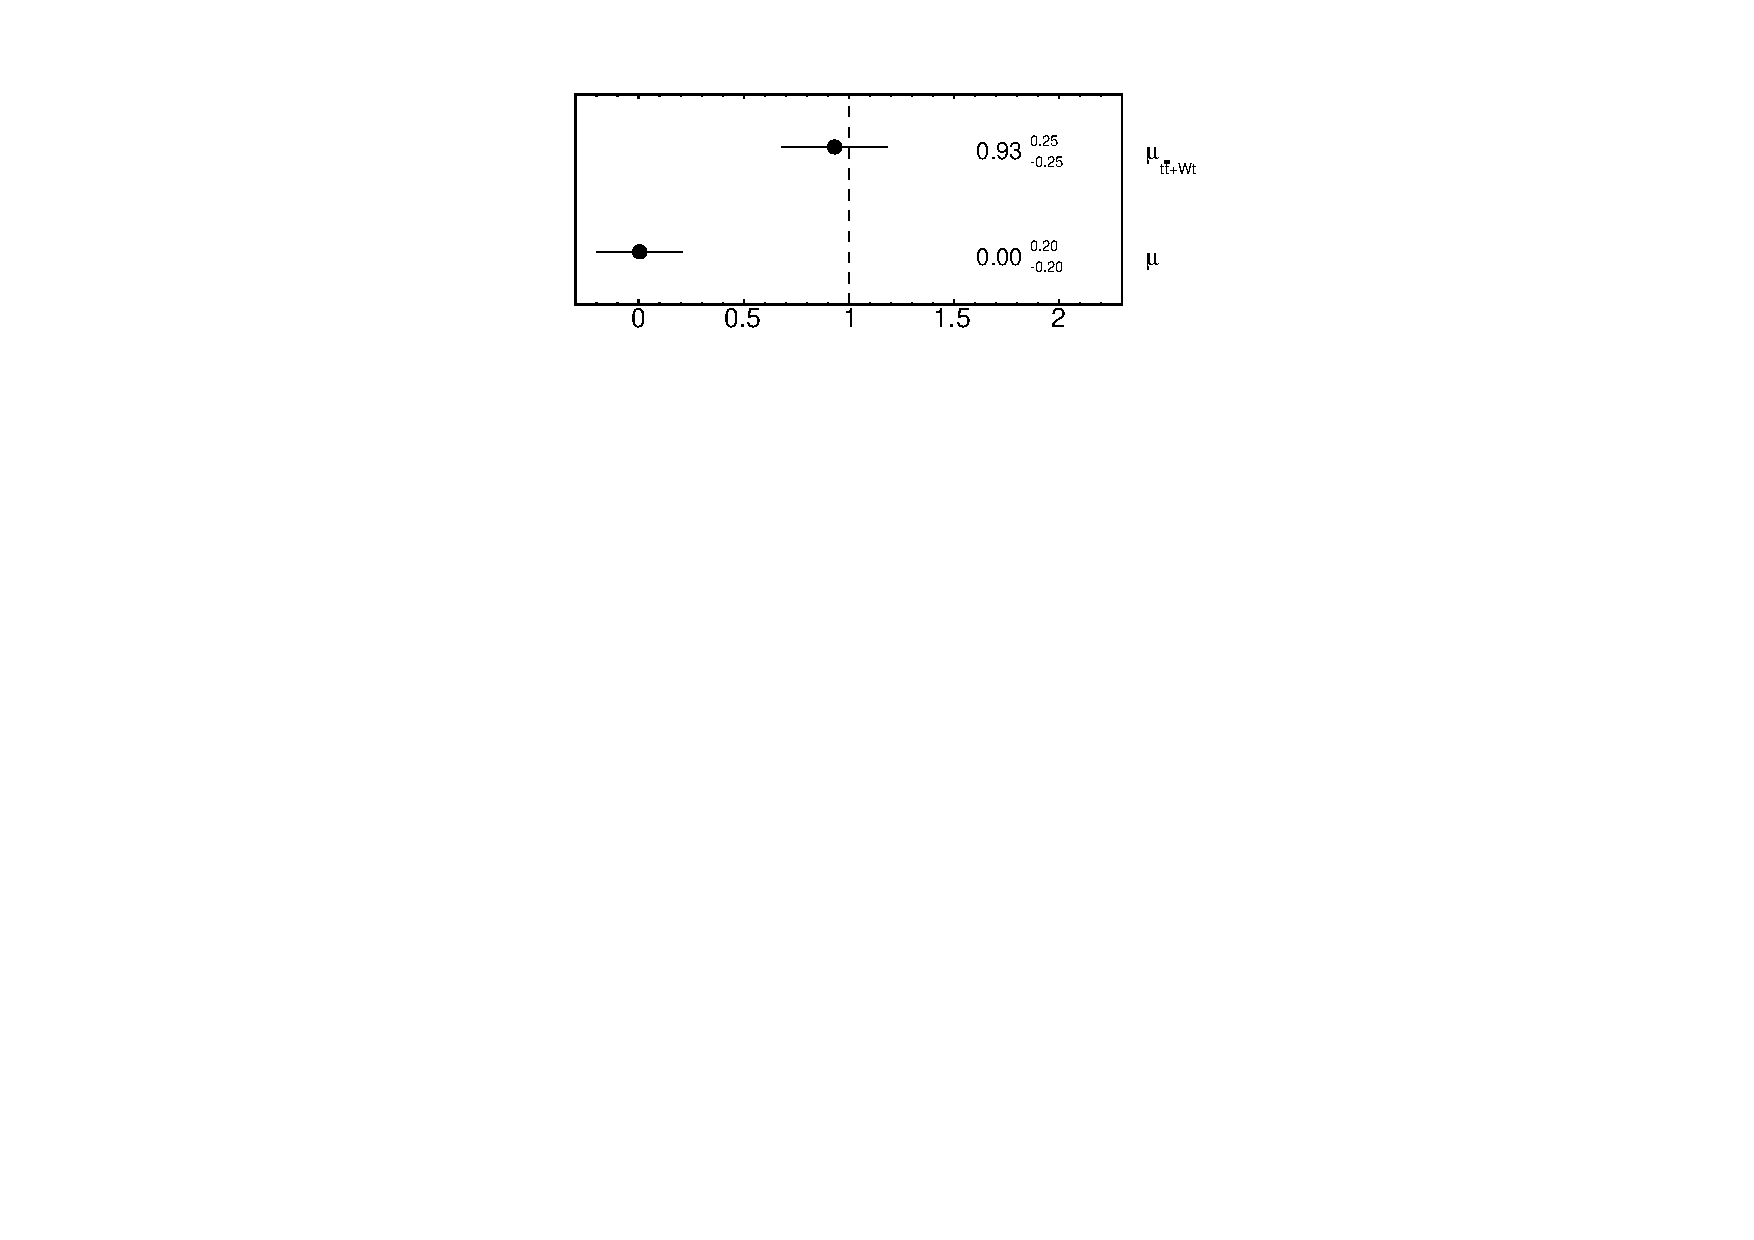
\includegraphics[width=.4\textwidth]{Appendices/AP9/figures/SPLUSB_CRSR_UsingBaseFullSys/NormFactors}
	\caption{Normalisation factors for the S+B \tZc fit in SRs+CRs with realistic Asimov.}%
	\label{fig:stat:tzc:splusb:crsr:norm_base}
\end{figure}
\restoregeometry

\begin{figure}[htbp]
	\centering
	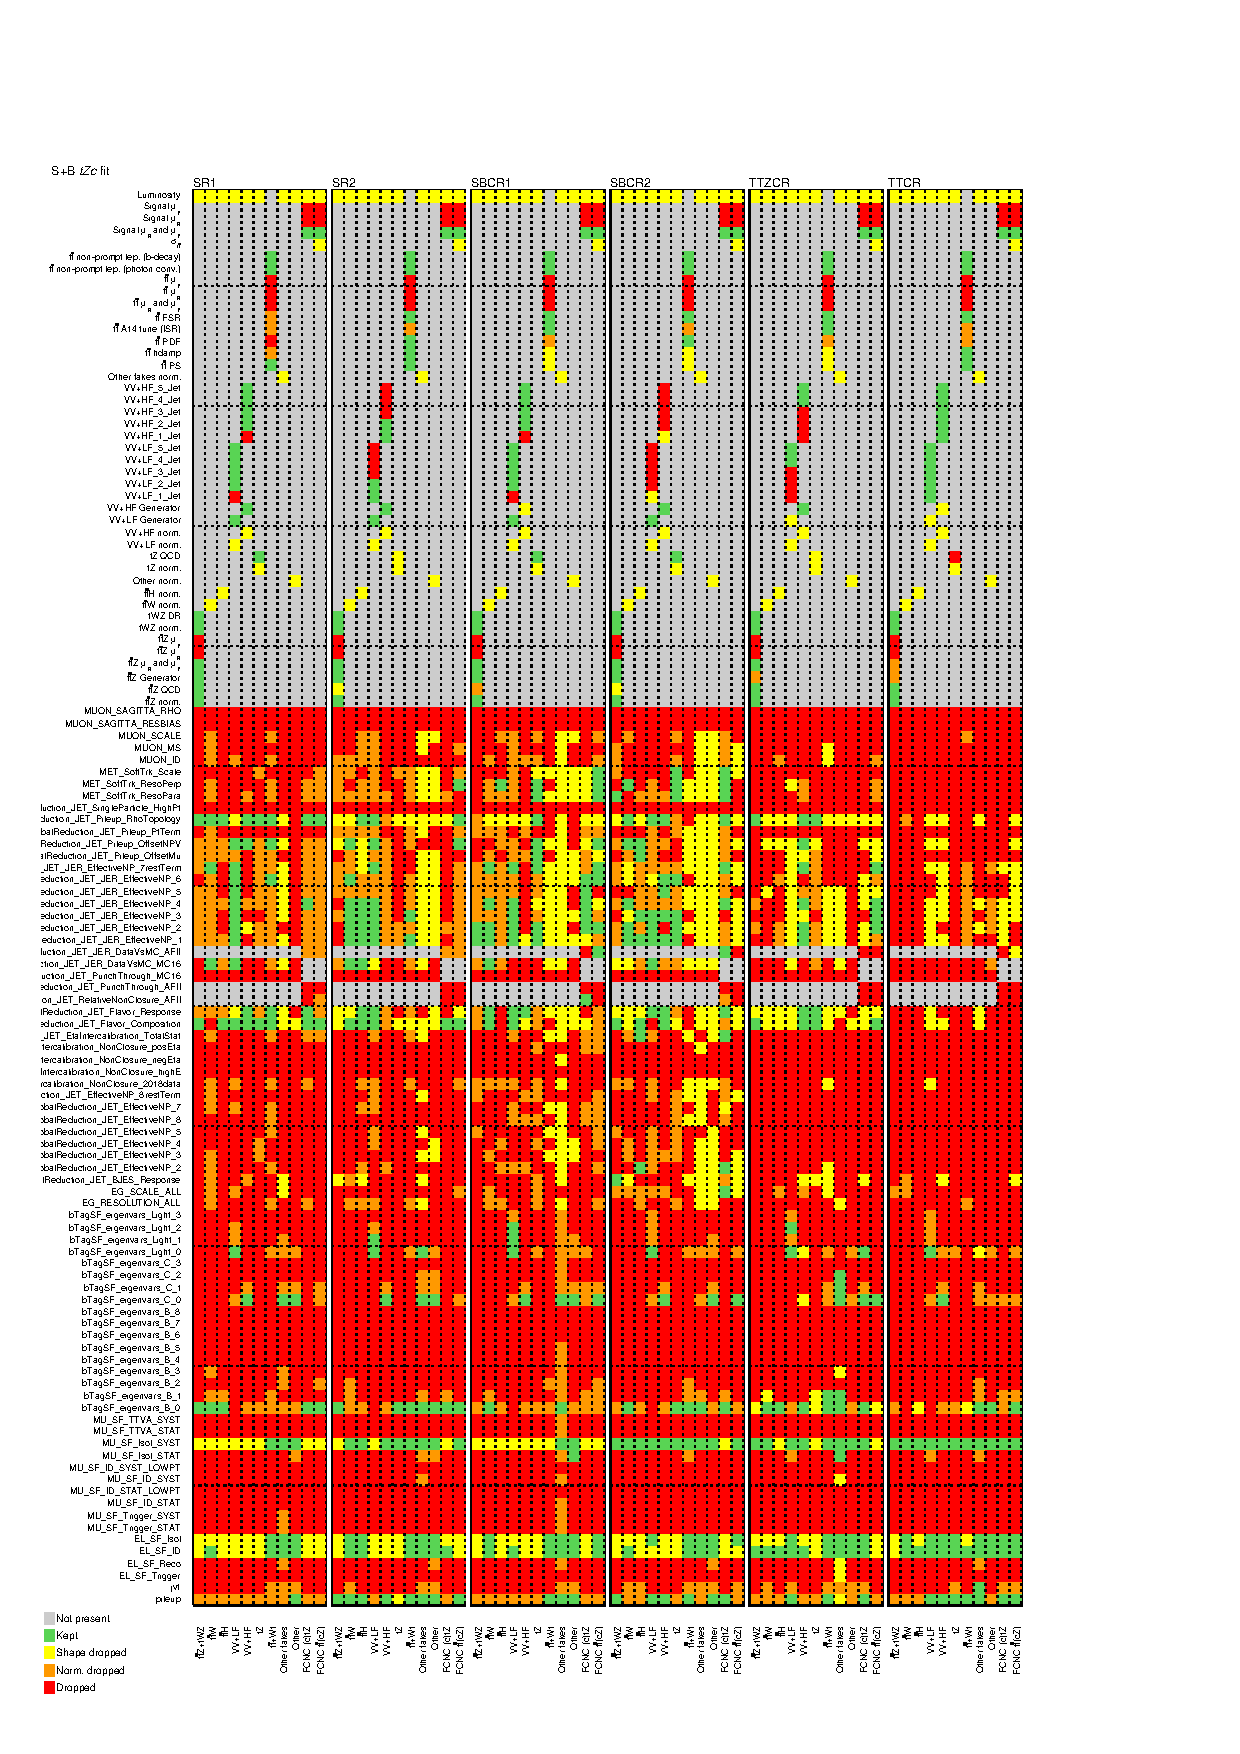
\includegraphics[width=.85\textwidth]{Appendices/AP9/figures/SPLUSB_CRSR_UsingBaseFullSys/Pruning}
	\caption{Pruning of the nuisance parameters for the S+B fit in SRs+CRs with realistic Asimov.}%
	\label{fig:stat:tzc:splusb:crsr:pruning_base}
\end{figure}

\begin{figure}[htbp]
	\centering
	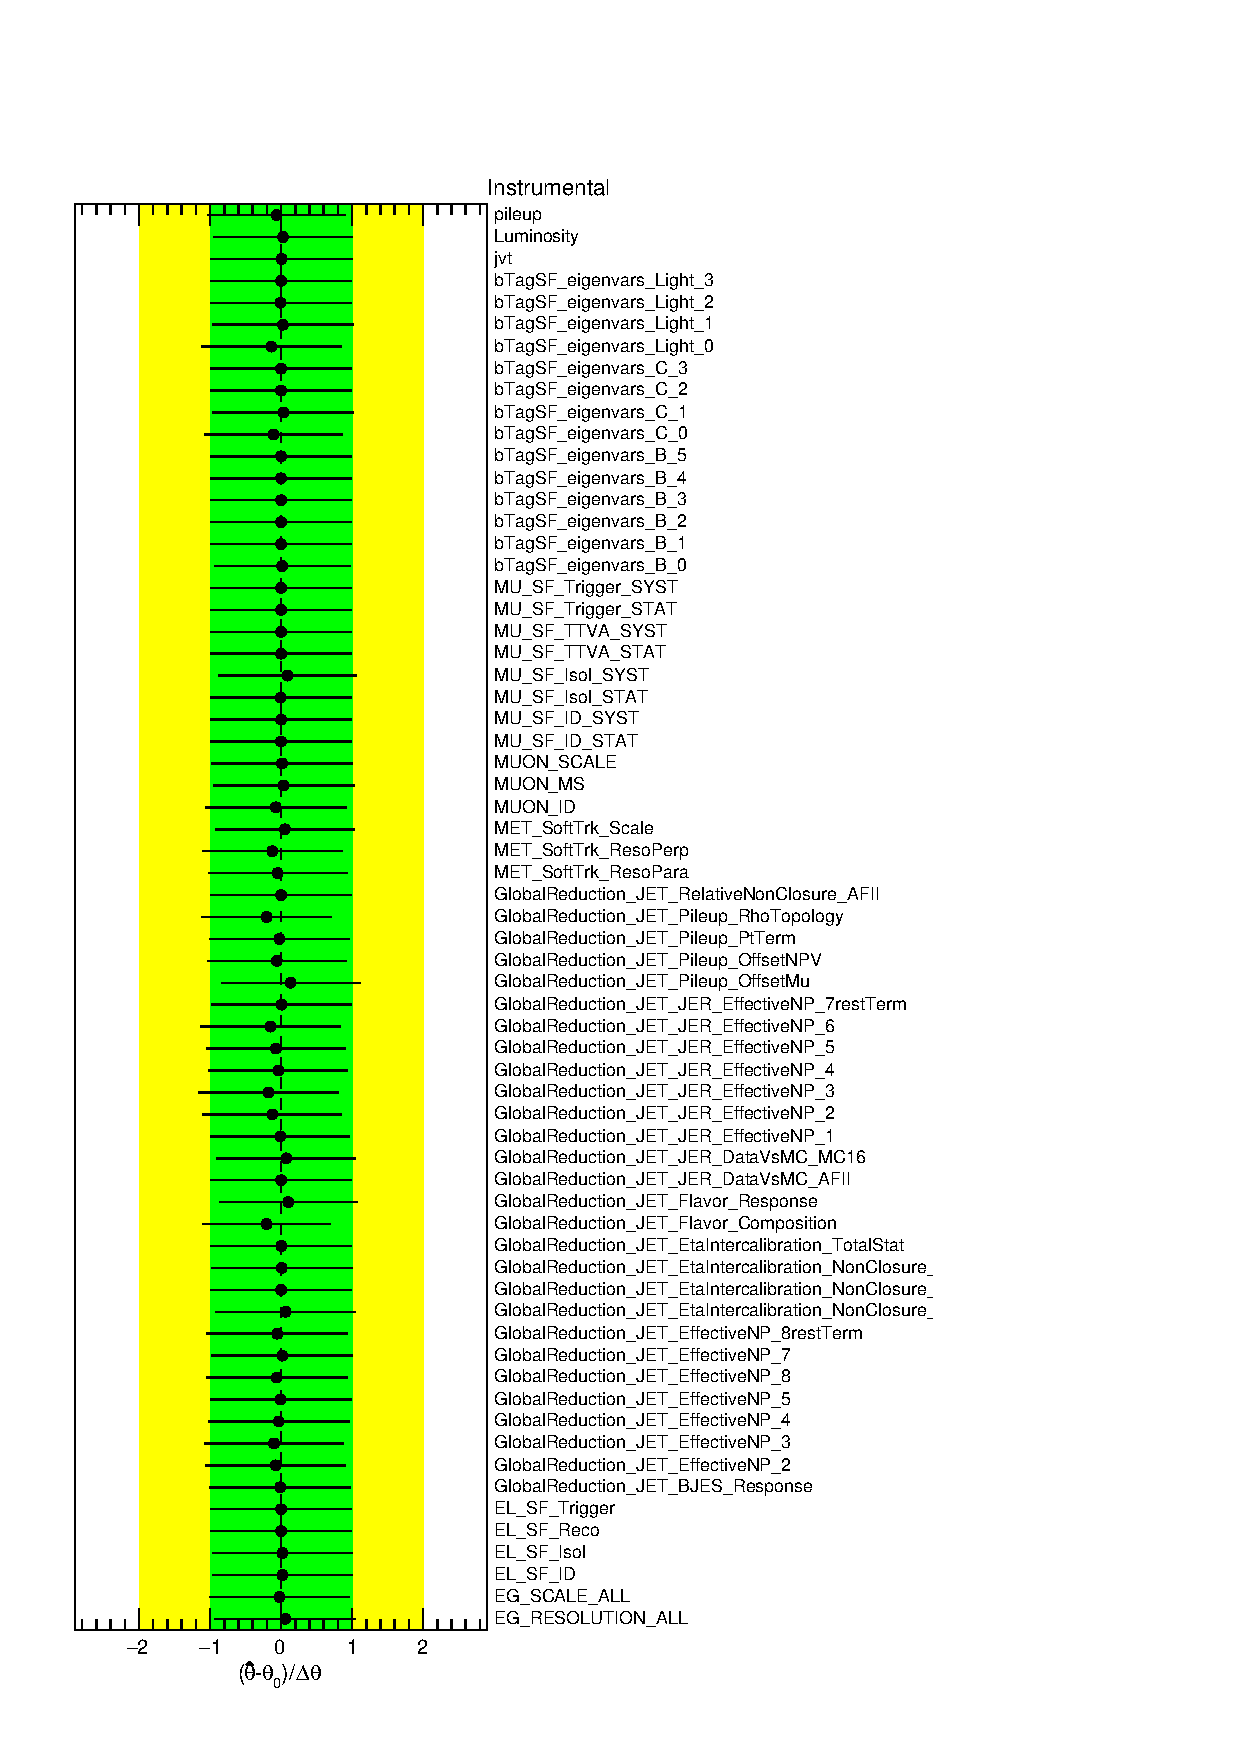
\includegraphics[width=.8\textwidth]{Appendices/AP9/figures/SPLUSB_CRSR_UsingBaseFullSys/NuisPar_Instrumental}
	\caption{Pulls and constraints of the instrumental nuisance parameters for the S+B \tZc fit in SRs+CRs with realistic Asimov.}%
	\label{fig:stat:tzc:splusb:crsr:np:instr_base}
\end{figure}

\begin{figure}[htbp]
	\centering
	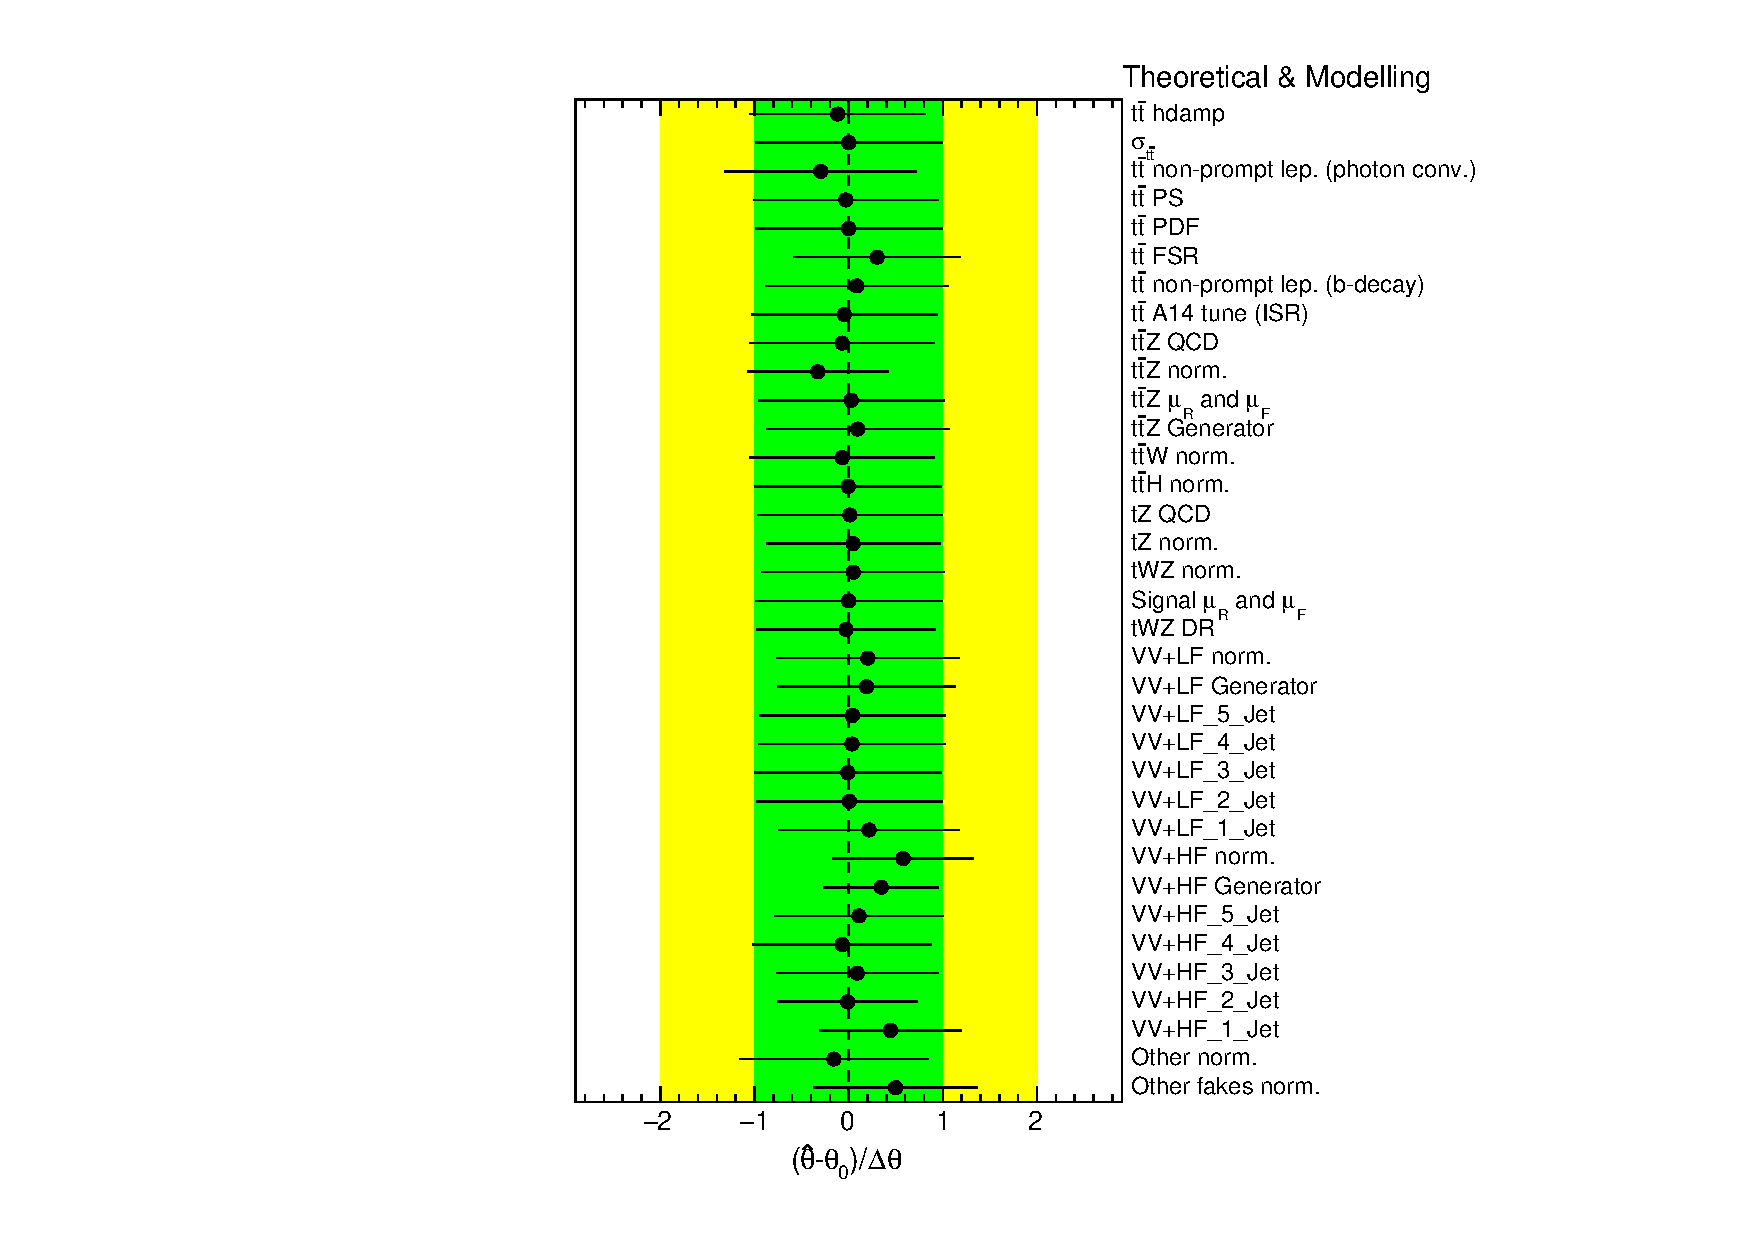
\includegraphics[width=.85\textwidth]{Appendices/AP9/figures/SPLUSB_CRSR_UsingBaseFullSys/NuisPar_Theoretical_&_Modelling}
	\caption{Pulls and constraints of the theoretical and modeling nuisance parameters for the S+B \tZc fit in SRs+CRs with realistic Asimov.}%
	\label{fig:stat:tzc:splusb:crsr:np:model_base}
\end{figure}

\begin{figure}[htbp]
	\centering
	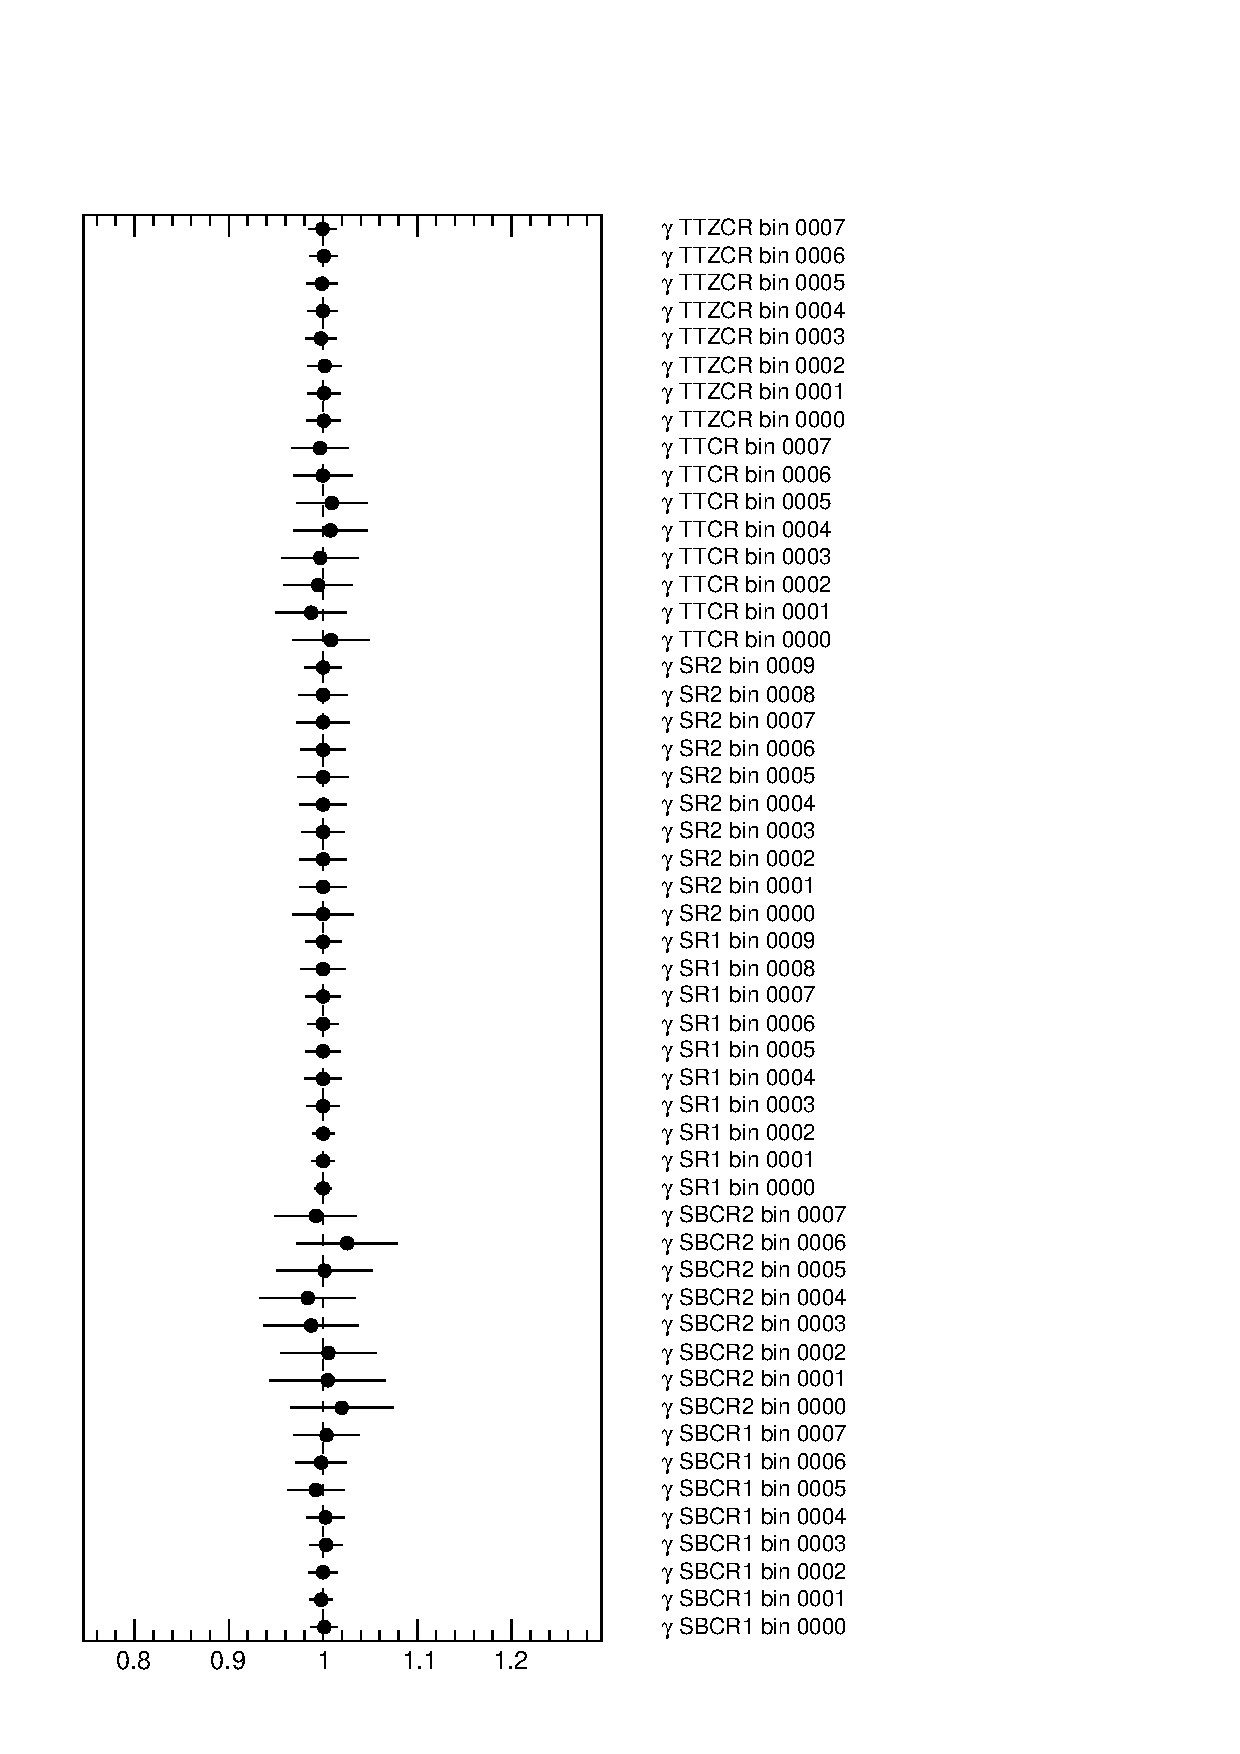
\includegraphics[width=.85\textwidth]{Appendices/AP9/figures/SPLUSB_CRSR_UsingBaseFullSys/Gammas}
	\caption{Gamma parameters for the S+B \tZc fit in SRs+CRs with realistic Asimov.}%
	\label{fig:stat:tzc:splusb:crsr:gamma_base}
\end{figure}

\begin{figure}[htbp]
	\centering
	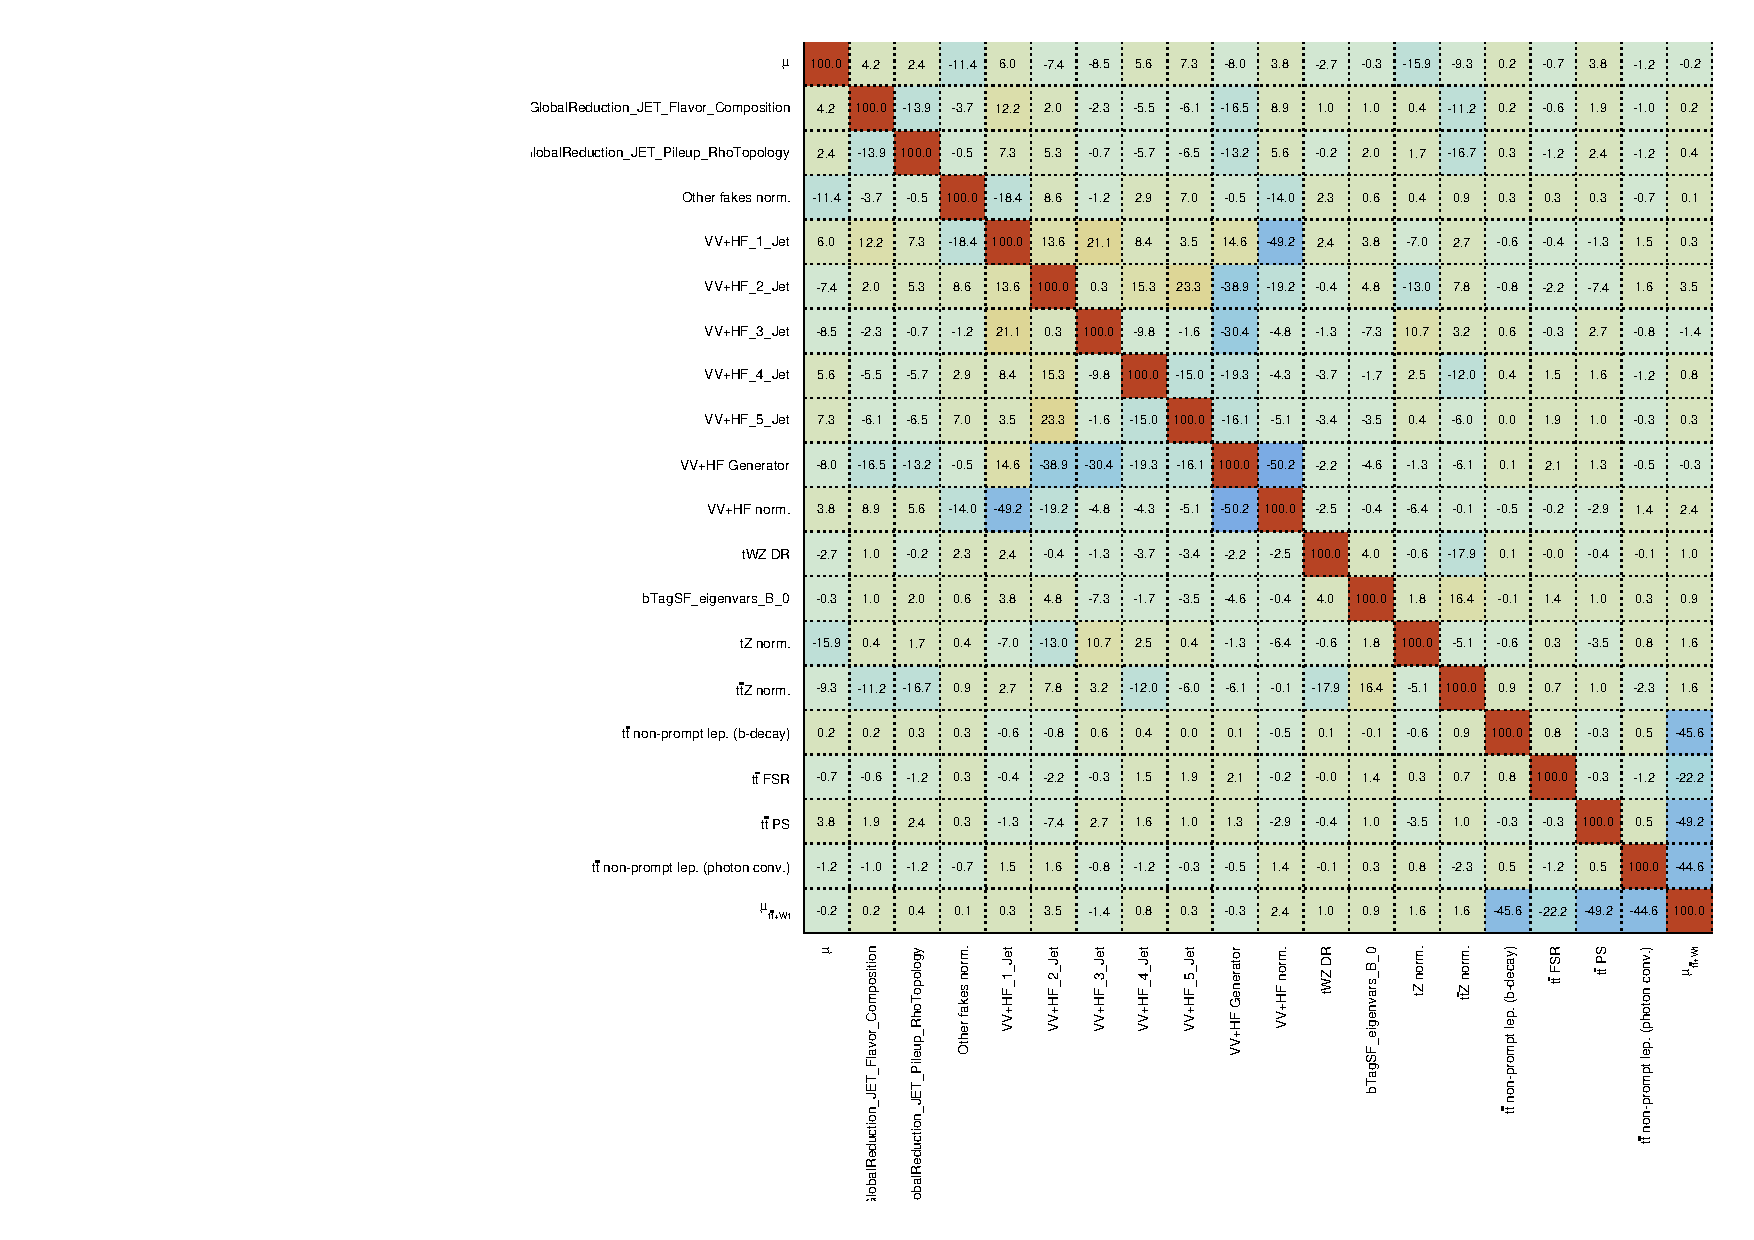
\includegraphics[width=.95\textwidth]{Appendices/AP9/figures/SPLUSB_CRSR_UsingBaseFullSys/CorrMatrix}
	\caption{Correlation matrix of the nuisance paramenters for the S+B \tZc fit in SRs+CRs with realistic Asimov.}%
	\label{fig:stat:tzc:splusb:crsr:corrmatrix_base}
\end{figure}

%\begin{figure}[htbp]
%	\centering
%	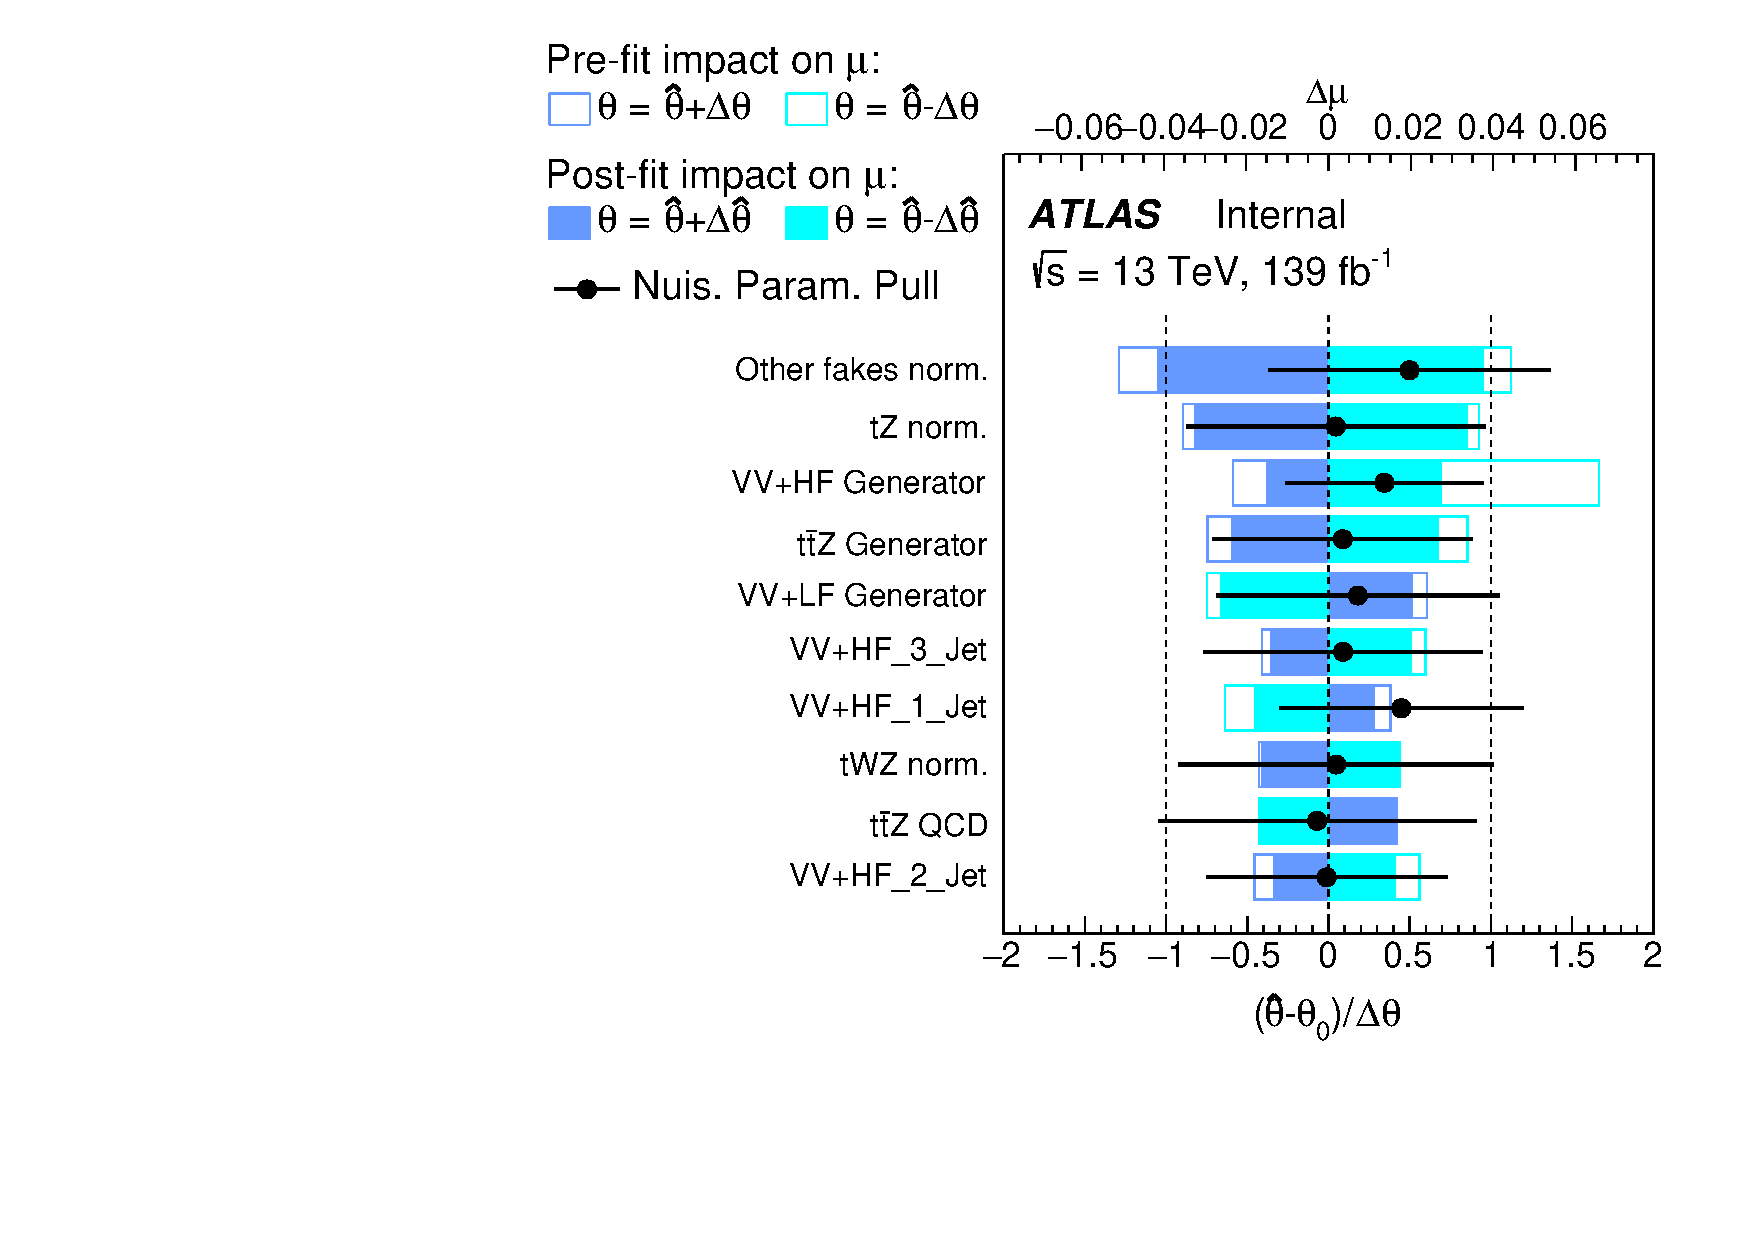
\includegraphics[width=.9\textwidth]{Appendices/AP9/figures/SPLUSB_CRSR_UsingBaseFullSys/Ranking}
%	\caption{Ranking of the nuisance parameters for the S+B \tZc fit in SRs+CRs with realistic Asimov.}%
%	\label{fig:stat:tzc:splusb:crsr:ranking_base}
%\end{figure}

\FloatBarrier
\clearpage
%\global\pdfpageattr\expandafter{\the\pdfpageattr/Rotate 90}
\begin{table}[]
	\centering
	\tiny
	% NB: add to main document: 
% NB: add to main document: 
% \usepackage{siunitx} 
% \sisetup{separate-uncertainty,table-format=6.3(6)}  % hint: modify table-format to best fit your tables
\begin{tabular}{|p{0.10\textwidth}|>{\centering}p{0.08\textwidth}|>{\centering}p{0.09\textwidth}|>{\centering}p{0.09\textwidth}|>{\centering}p{0.09\textwidth}|>{\centering}p{0.09\textwidth}|>{\centering\arraybackslash}p{0.09\textwidth}|}
	\toprule  
	& {SR1tZc} & {SR2tZc} & {Side-band CR1} & {Side-band CR2} & {\ttZ CR} & {\ttbar CR}\\
	\midrule 
	\ttZ+\tWZ   & 208 $\pm$ 27 & 36 $\pm$ 7 & 88 $\pm$ 12 & 9.1 $\pm$ 2.1 & 164 $\pm$ 22 & 14.8 $\pm$ 1.9 \\ 
	\ttW   & 6.8 $\pm$ 1.1 & 3.6 $\pm$ 0.6 & 4.3 $\pm$ 0.7 & 2.5 $\pm$ 0.5 & 2.3 $\pm$ 0.4 & 27 $\pm$ 4 \\ 
	\ttH   & 7.8 $\pm$ 1.2 & 0.95 $\pm$ 0.18 & 2.3 $\pm$ 0.4 & 0.36 $\pm$ 0.07 & 5.4 $\pm$ 0.9 & 13.8 $\pm$ 2.1 \\ 
	\VVLF   & 29 $\pm$ 18 & 35 $\pm$ 13 & 25 $\pm$ 15 & 18 $\pm$ 7 & 0.20 $\pm$ 0.22 & 0.40 $\pm$ 0.20 \\ 
	\VVHF   & 150 $\pm$ 110 & 160 $\pm$ 70 & 130 $\pm$ 80 & 69 $\pm$ 28 & 13 $\pm$ 11 & 2.3 $\pm$ 1.4 \\ 
	\tZq   & 51 $\pm$ 8 & 113 $\pm$ 18 & 20 $\pm$ 4 & 9.9 $\pm$ 1.7 & 14.6 $\pm$ 2.8 & 0.90 $\pm$ 0.15 \\ 
	\ttbar+Wt   & 22 $\pm$ 5 & 33 $\pm$ 12 & 10 $\pm$ 4 & 9.1 $\pm$ 2.7 & 3.0 $\pm$ 1.2 & 102 $\pm$ 24 \\ 
	Other fakes   & 12 $\pm$ 12 & 12 $\pm$ 12 & 3 $\pm$ 5 & 10 $\pm$ 11 & 0.00 $\pm$ 0.06 & 0.12 $\pm$ 0.14 \\ 
	Other   & 2.7 $\pm$ 1.5 & 3.8 $\pm$ 2.8 & 2.2 $\pm$ 1.6 & 0.8 $\pm$ 2.6 & 1.1 $\pm$ 0.5 & 2.9 $\pm$ 1.5 \\ 
	FCNC (c)tZ   & 3.57 $\pm$ 0.27 & 12.1 $\pm$ 0.6 & 1.06 $\pm$ 0.12 & 0.83 $\pm$ 0.09 & 0.24 $\pm$ 0.04 & 0.083 $\pm$ 0.012 \\ 
	FCNC \ttbar(cZ)   & 76 $\pm$ 6 & 18.5 $\pm$ 1.9 & 4.2 $\pm$ 0.6 & 1.9 $\pm$ 0.4 & 3.7 $\pm$ 0.5 & 0.37 $\pm$ 0.06 \\ 
	\midrule 
	Total background  & 490 $\pm$ 120 & 400 $\pm$ 80 & 280 $\pm$ 80 & 130 $\pm$ 32 & 203 $\pm$ 26 & 164 $\pm$ 25 \\ 
	\midrule 
	Data   & 556 & 462 & 331 & 169 & 197 & 156 \\ 
	\midrule 
	Data / Bkg.   & 1.12 $\pm$ 0.27 & 1.17 $\pm$ 0.24 & 1.18 $\pm$ 0.35 & 1.30 $\pm$ 0.34 & 0.97 $\pm$ 0.14 & 0.95 $\pm$ 0.16 \\ 
	\bottomrule 
\end{tabular} 

	\caption{Pre-fit event yields in the S+B \tZc fit in SRs+CRs with realistic Asimov. \TabErrStatSys} 
	\label{tab:stat:tzc:splusb:crsr:yields:prefit_base}
\end{table} 

\begin{table}[]
	\centering
	\tiny
	\begin{tabular}{|p{0.10\textwidth}|>{\centering}p{0.08\textwidth}|>{\centering}p{0.09\textwidth}|>{\centering}p{0.09\textwidth}|>{\centering}p{0.09\textwidth}|>{\centering}p{0.09\textwidth}|>{\centering\arraybackslash}p{0.09\textwidth}|}
	\toprule  
	& {SR1tZc} & {SR2tZc} & {Side-band CR1} & {Side-band CR2} & {\ttZ CR} & {\ttbar CR}\\
	\midrule 
	\ttZ+\tWZ   & 201 $\pm$ 19 & 37 $\pm$ 7 & 86 $\pm$ 9 & 9.3 $\pm$ 2.0 & 157 $\pm$ 13 & 14.4 $\pm$ 1.4 \\ 
	\ttW   & 6.7 $\pm$ 1.1 & 3.6 $\pm$ 0.6 & 4.2 $\pm$ 0.7 & 2.5 $\pm$ 0.5 & 2.2 $\pm$ 0.4 & 26 $\pm$ 4 \\ 
	\ttH   & 7.8 $\pm$ 1.2 & 0.97 $\pm$ 0.18 & 2.3 $\pm$ 0.4 & 0.37 $\pm$ 0.07 & 5.3 $\pm$ 0.8 & 13.8 $\pm$ 2.1 \\ 
	\VVLF   & 33 $\pm$ 19 & 39 $\pm$ 14 & 29 $\pm$ 16 & 21 $\pm$ 8 & 0.24 $\pm$ 0.23 & 0.40 $\pm$ 0.18 \\ 
	\VVHF   & 220 $\pm$ 40 & 216 $\pm$ 30 & 172 $\pm$ 25 & 94 $\pm$ 16 & 18 $\pm$ 6 & 3.3 $\pm$ 0.5 \\ 
	\tZq   & 51 $\pm$ 7 & 115 $\pm$ 17 & 19.6 $\pm$ 3.3 & 10.1 $\pm$ 1.6 & 14.4 $\pm$ 2.5 & 0.91 $\pm$ 0.12 \\ 
	\ttbar+Wt   & 20 $\pm$ 4 & 31 $\pm$ 7 & 9.5 $\pm$ 2.8 & 8.6 $\pm$ 1.6 & 2.5 $\pm$ 0.8 & 95 $\pm$ 13 \\ 
	Other fakes   & 17 $\pm$ 12 & 17 $\pm$ 13 & 5 $\pm$ 5 & 18 $\pm$ 14 & 0.005 $\pm$ 0.009 & 0.18 $\pm$ 0.13 \\ 
	Other   & 2.5 $\pm$ 1.3 & 3.7 $\pm$ 2.5 & 1.8 $\pm$ 1.2 & 0.2 $\pm$ 0.9 & 1.0 $\pm$ 0.5 & 2.7 $\pm$ 1.4 \\ 
	FCNC (c)tZ   & 0.0 $\pm$ 0.7 & 0.1 $\pm$ 2.5 & 0.00 $\pm$ 0.21 & 0.00 $\pm$ 0.17 & 0.00 $\pm$ 0.05 & 0.000 $\pm$ 0.017 \\ 
	FCNC \ttbar(cZ)   & 0 $\pm$ 16 & 0 $\pm$ 4 & 0.0 $\pm$ 0.9 & 0.0 $\pm$ 0.4 & 0.0 $\pm$ 0.7 & 0.00 $\pm$ 0.07 \\ 
	\midrule 
	Total background  & 556 $\pm$ 25 & 462 $\pm$ 21 & 328 $\pm$ 17 & 165 $\pm$ 13 & 201 $\pm$ 12 & 157 $\pm$ 12 \\ 
	\midrule 
	Data   & 556 & 462 & 331 & 169 & 197 & 156 \\ 
	\midrule 
	Data / Bkg.   & 1.00 $\pm$ 0.04 & 1.00 $\pm$ 0.05 & 1.01 $\pm$ 0.05 & 1.02 $\pm$ 0.08 & 0.98 $\pm$ 0.06 & 0.99 $\pm$ 0.08 \\ 
	\bottomrule 
\end{tabular} 

	\caption{Post-fit event yields in the S+B\tZc fit in SRs+CRs with realistic Asimov. \TabErrStatSys} 
	\label{tab:stat:tzc:splusb:crsr:yields:postfit_base}
\end{table} 
\clearpage
\FloatBarrier
%\global\pdfpageattr\expandafter{\the\pdfpageattr/Rotate 0}

\clearpage
\begin{figure}[htbp]
	\centering
	\begin{tabular}{cc}
		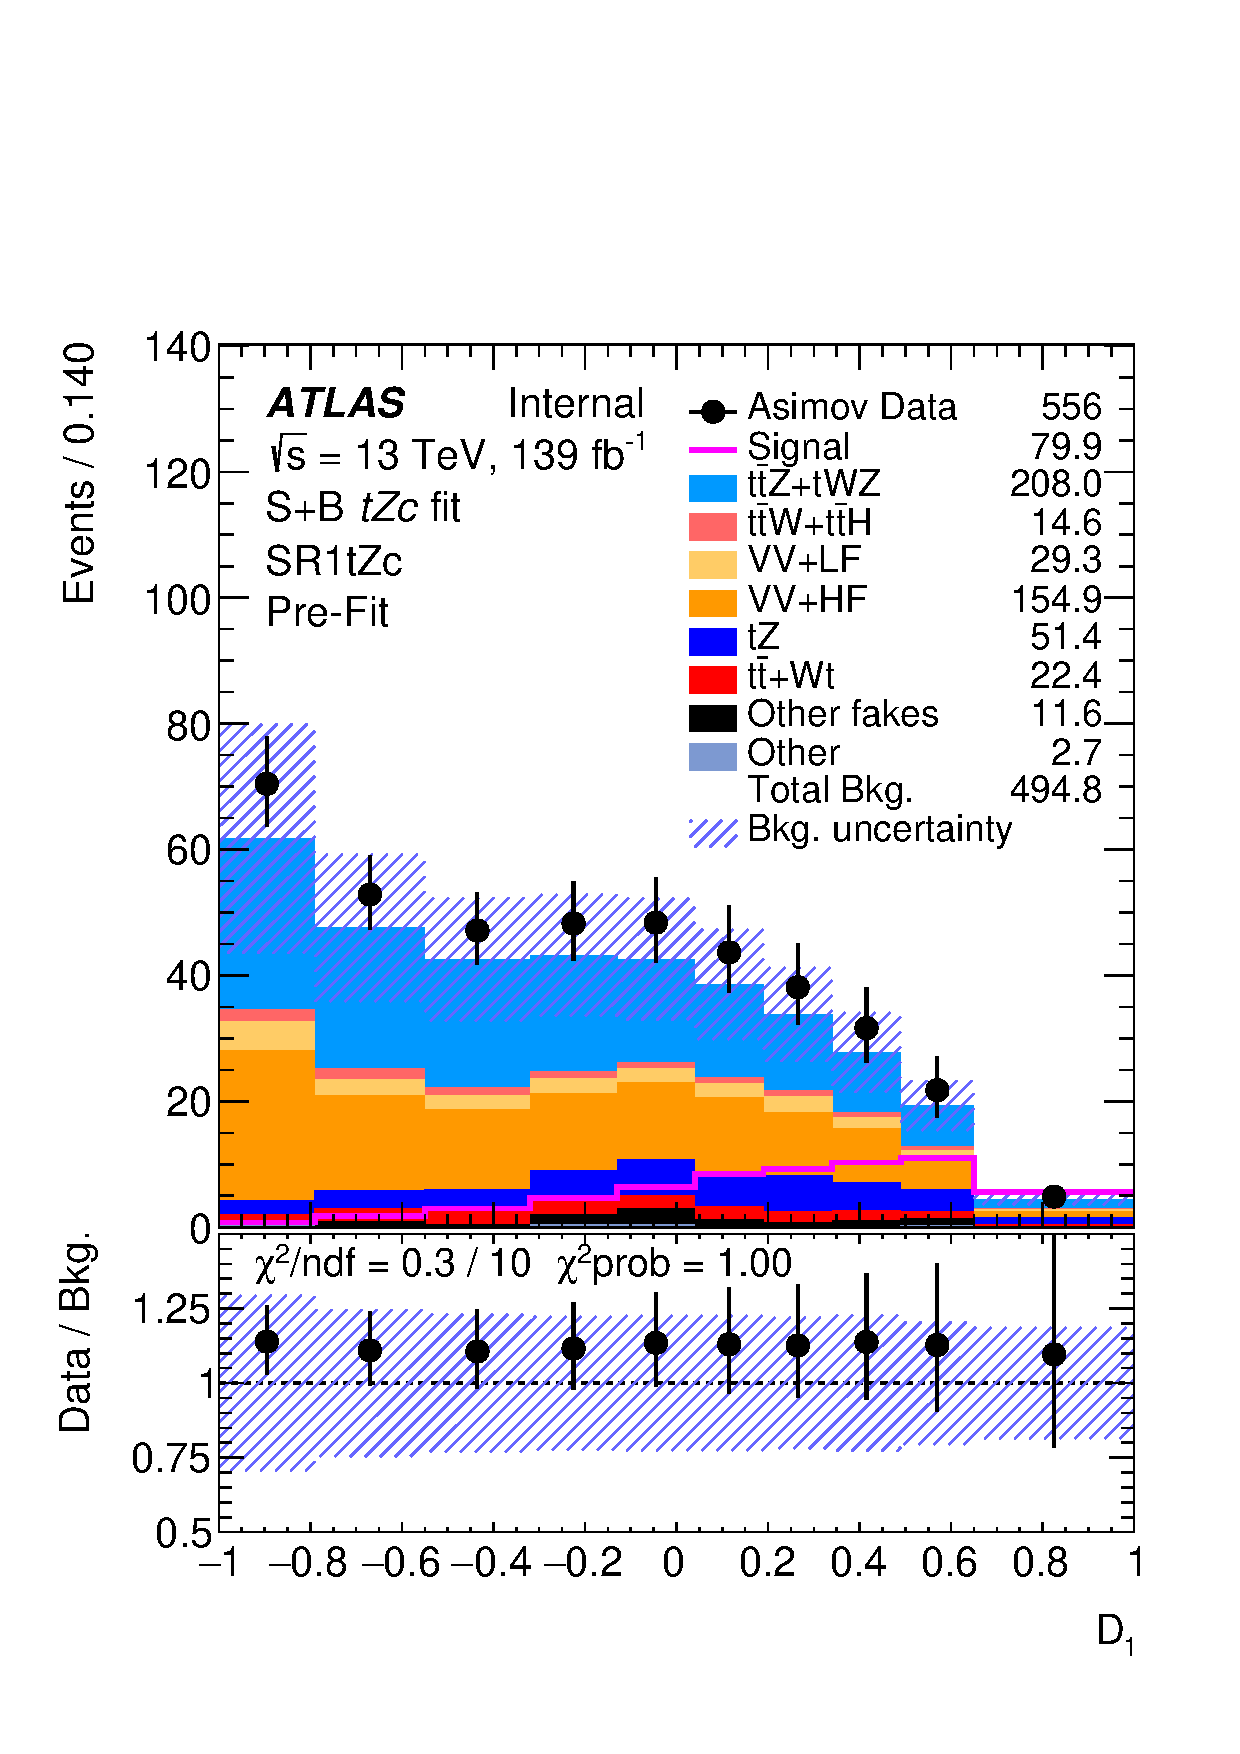
\includegraphics[width=.45\textwidth]{Appendices/AP9/figures/SPLUSB_CRSR_UsingBaseFullSys/Plots/SR1} &
		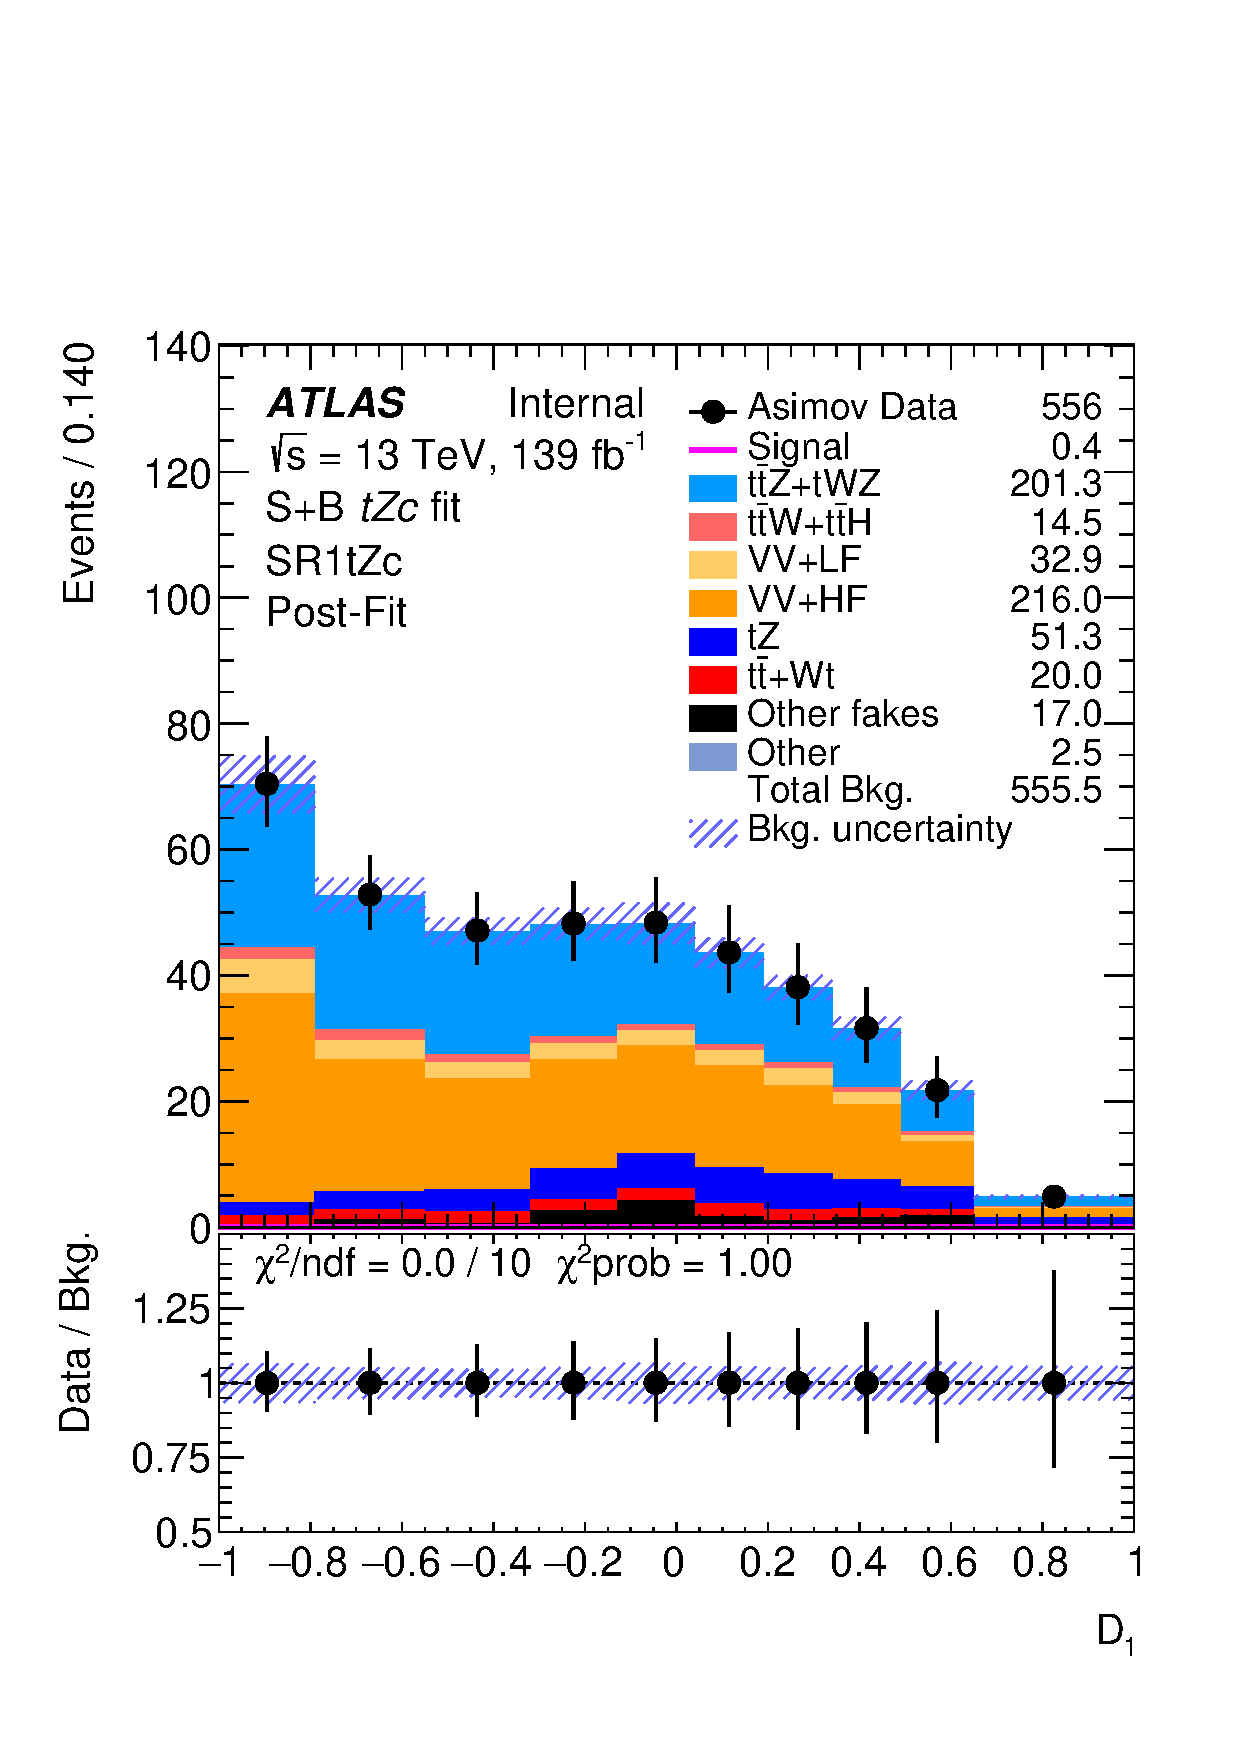
\includegraphics[width=.45\textwidth]{Appendices/AP9/figures/SPLUSB_CRSR_UsingBaseFullSys/Plots/SR1_postFit} \\
		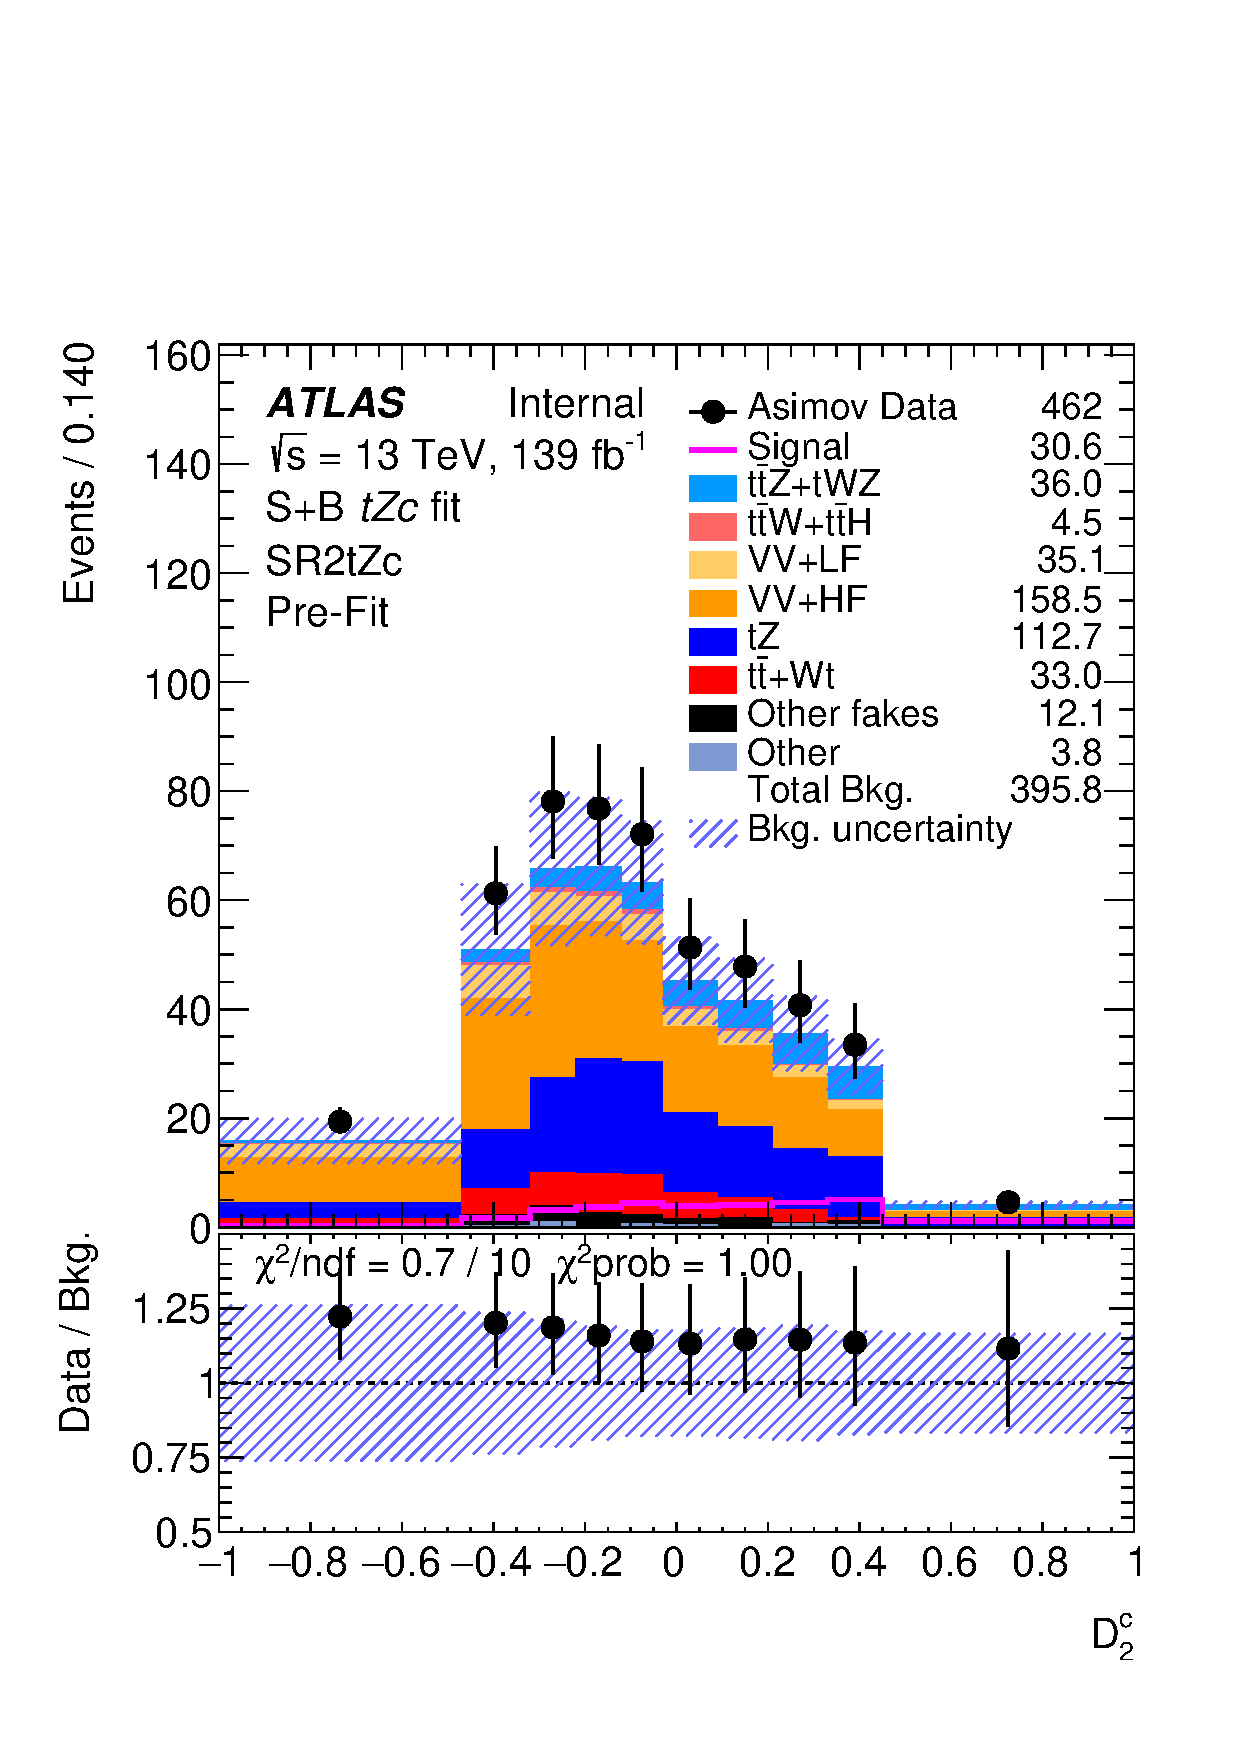
\includegraphics[width=.45\textwidth]{Appendices/AP9/figures/SPLUSB_CRSR_UsingBaseFullSys/Plots/SR2} &
		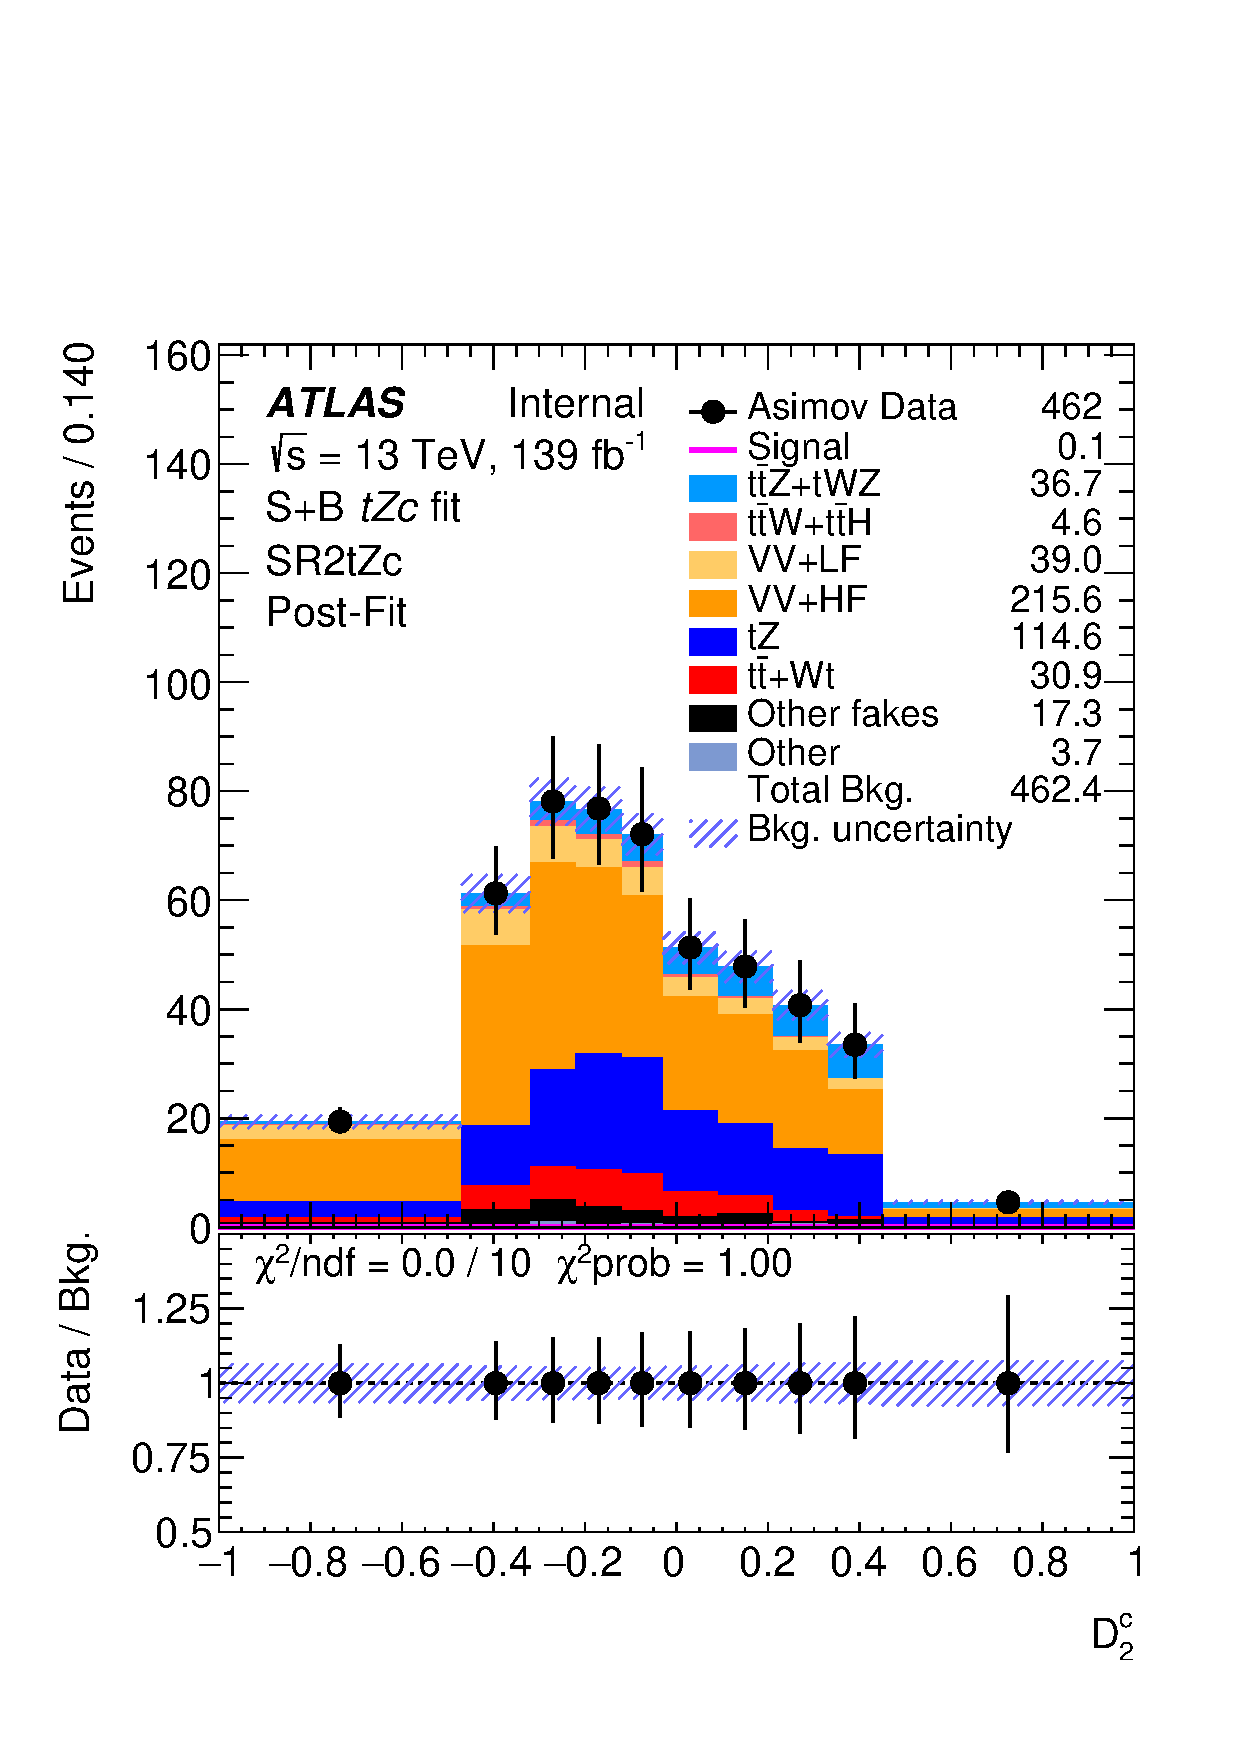
\includegraphics[width=.45\textwidth]{Appendices/AP9/figures/SPLUSB_CRSR_UsingBaseFullSys/Plots/SR2_postFit} \\
	\end{tabular}
	\caption{Pre-fit (left) and post-fit (right) BDTG output distributions in SR1 and SR2 for the S+B \tZc fit in SRs+CRs with realistic Asimov.
		\ErrStatSys
	}%
	\label{fig:stat:tzc:splusb:crsr:srplots:1_base}
\end{figure}

\begin{figure}[htbp]
	\centering
	\begin{tabular}{cc}
		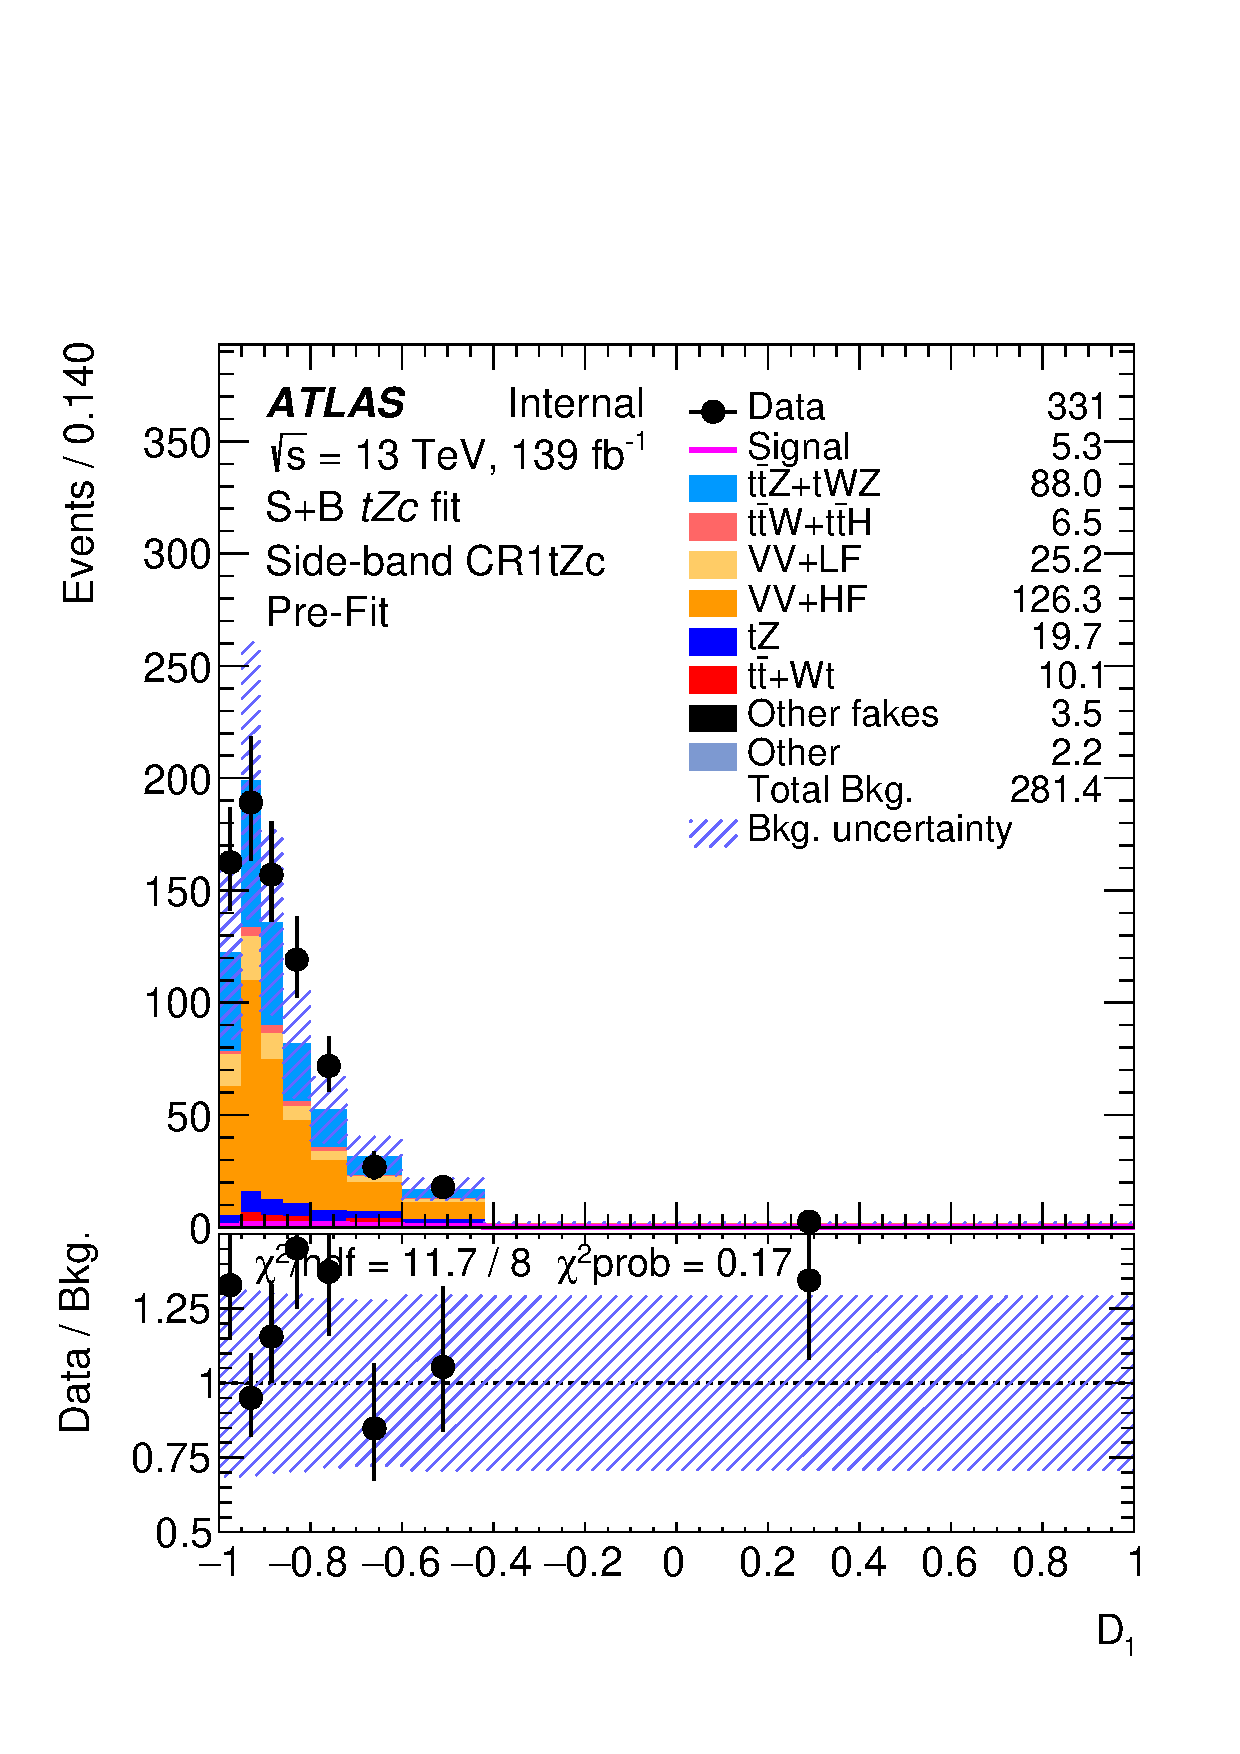
\includegraphics[width=.45\textwidth]{Appendices/AP9/figures/SPLUSB_CRSR_UsingBaseFullSys/Plots/SBCR1} &
		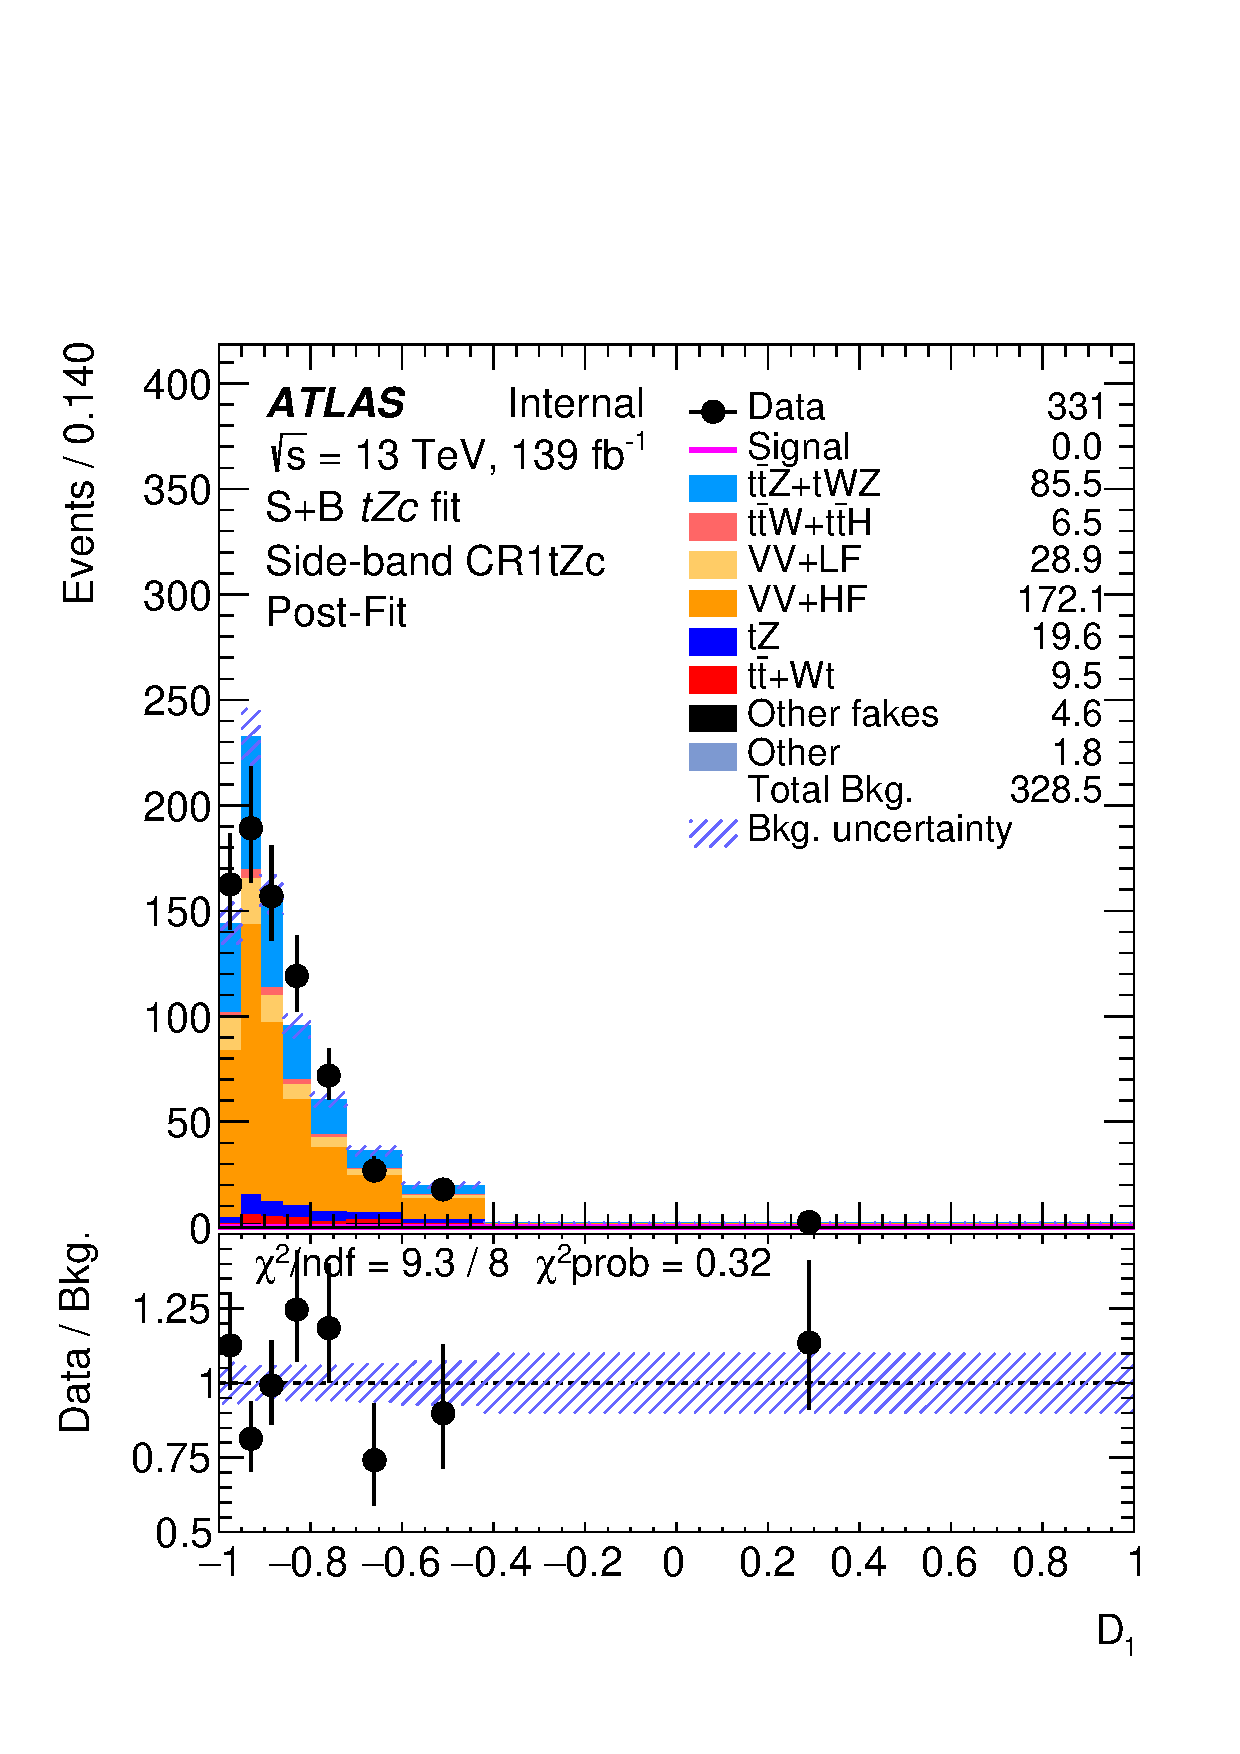
\includegraphics[width=.45\textwidth]{Appendices/AP9/figures/SPLUSB_CRSR_UsingBaseFullSys/Plots/SBCR1_postFit} \\
		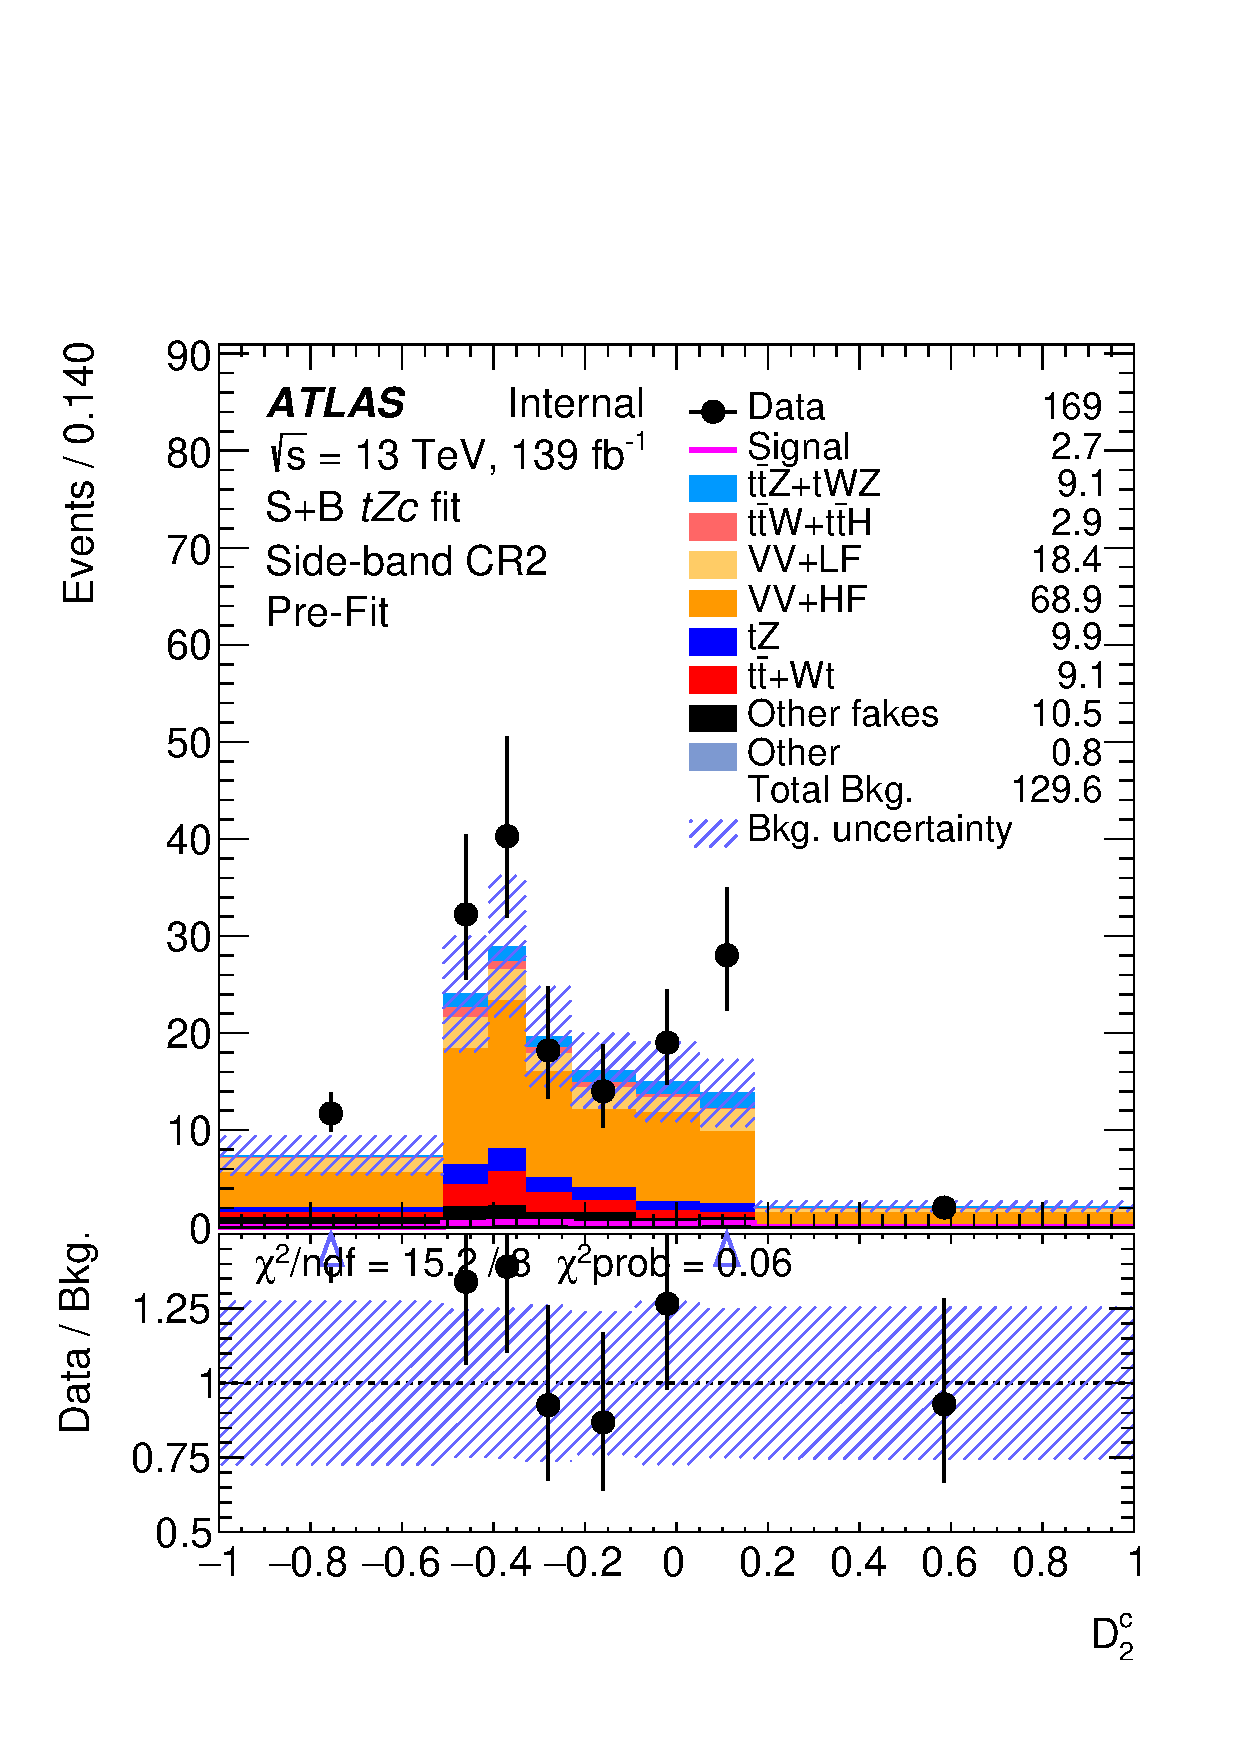
\includegraphics[width=.45\textwidth]{Appendices/AP9/figures/SPLUSB_CRSR_UsingBaseFullSys/Plots/SBCR2} &
		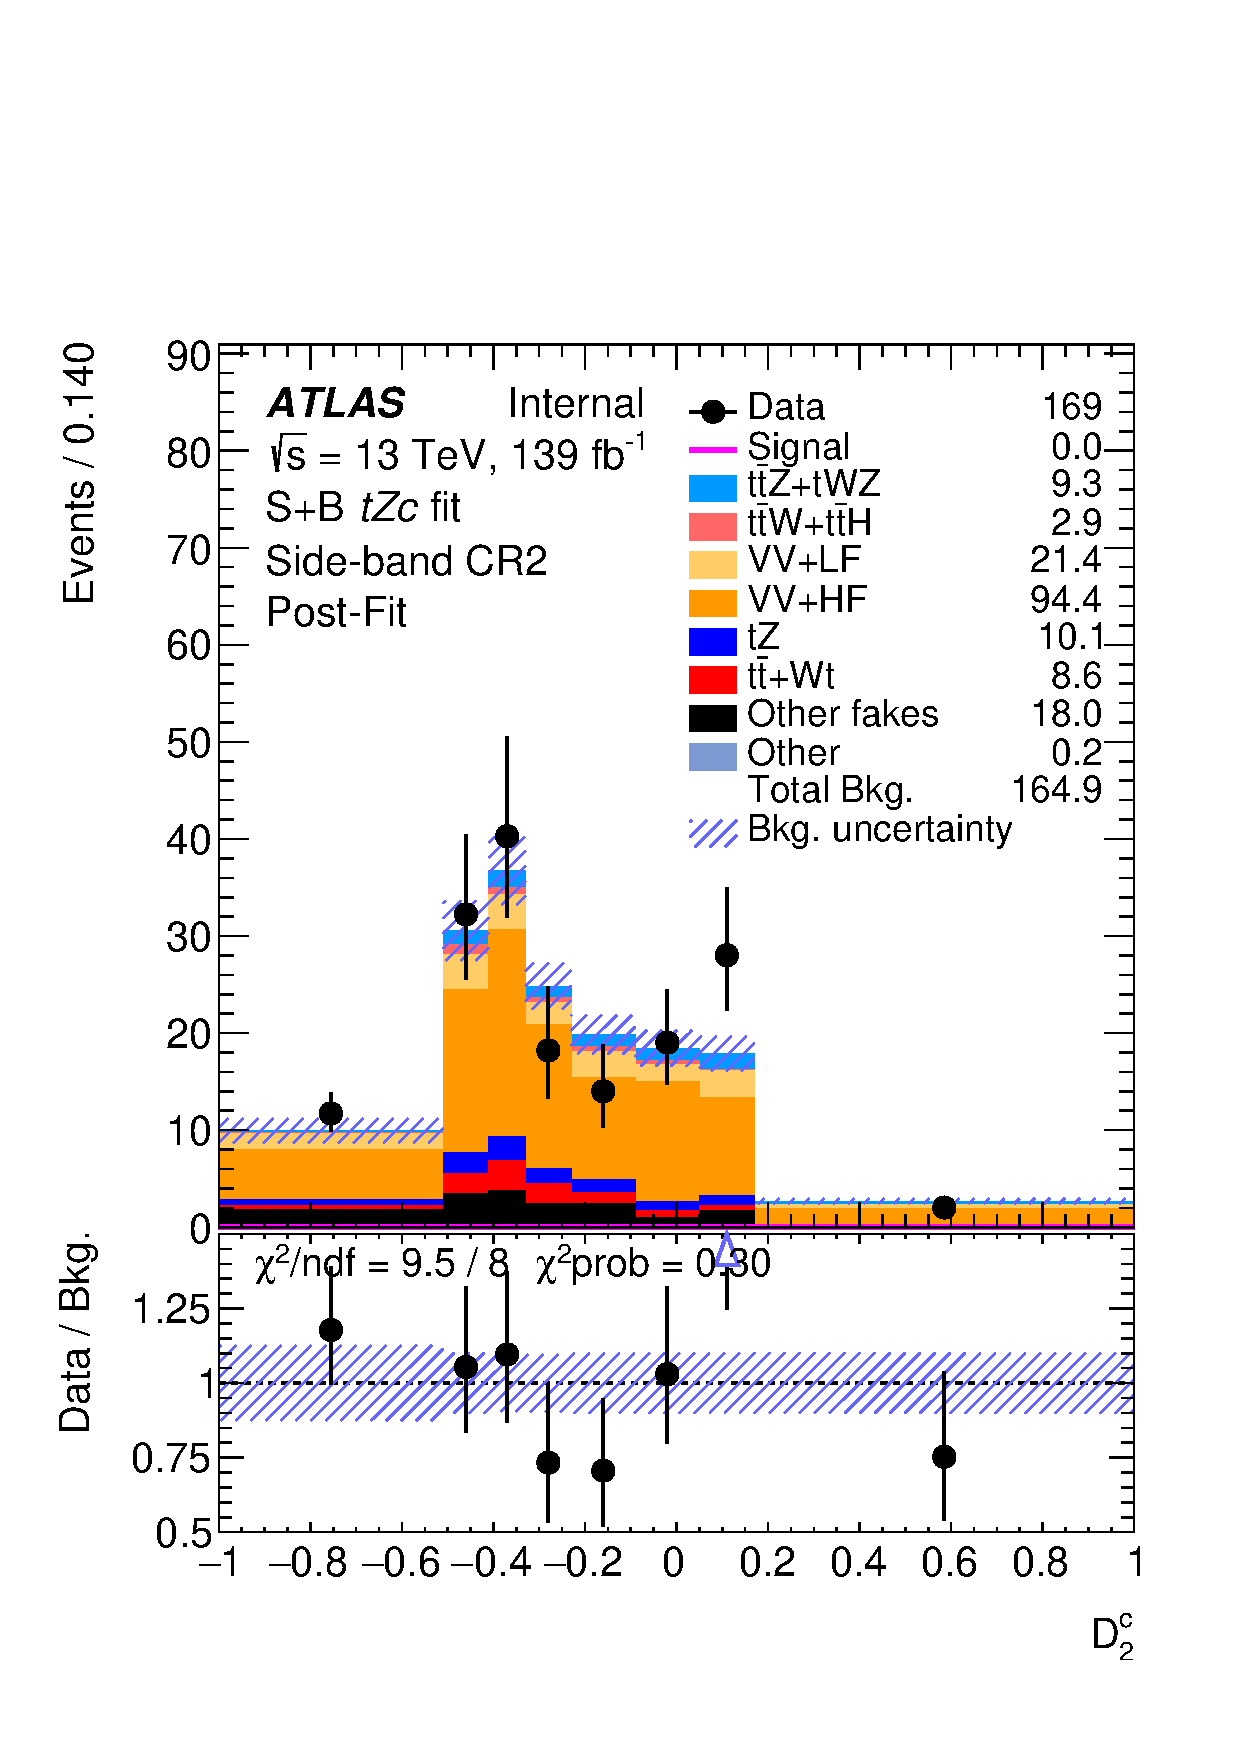
\includegraphics[width=.45\textwidth]{Appendices/AP9/figures/SPLUSB_CRSR_UsingBaseFullSys/Plots/SBCR2_postFit} \\
	\end{tabular}
	\caption{Pre-fit (left) and post-fit (right) BDTG output distributions in the side-band CRs for the S+B \tZc fit in SRs+CRs with realistic Asimov.
		\ErrStatSys
	}%
	\label{fig:stat:tzc:splusb:crsr:crplots:1_base}
\end{figure}

\begin{figure}[htbp]
	\centering
	\begin{tabular}{cc}
		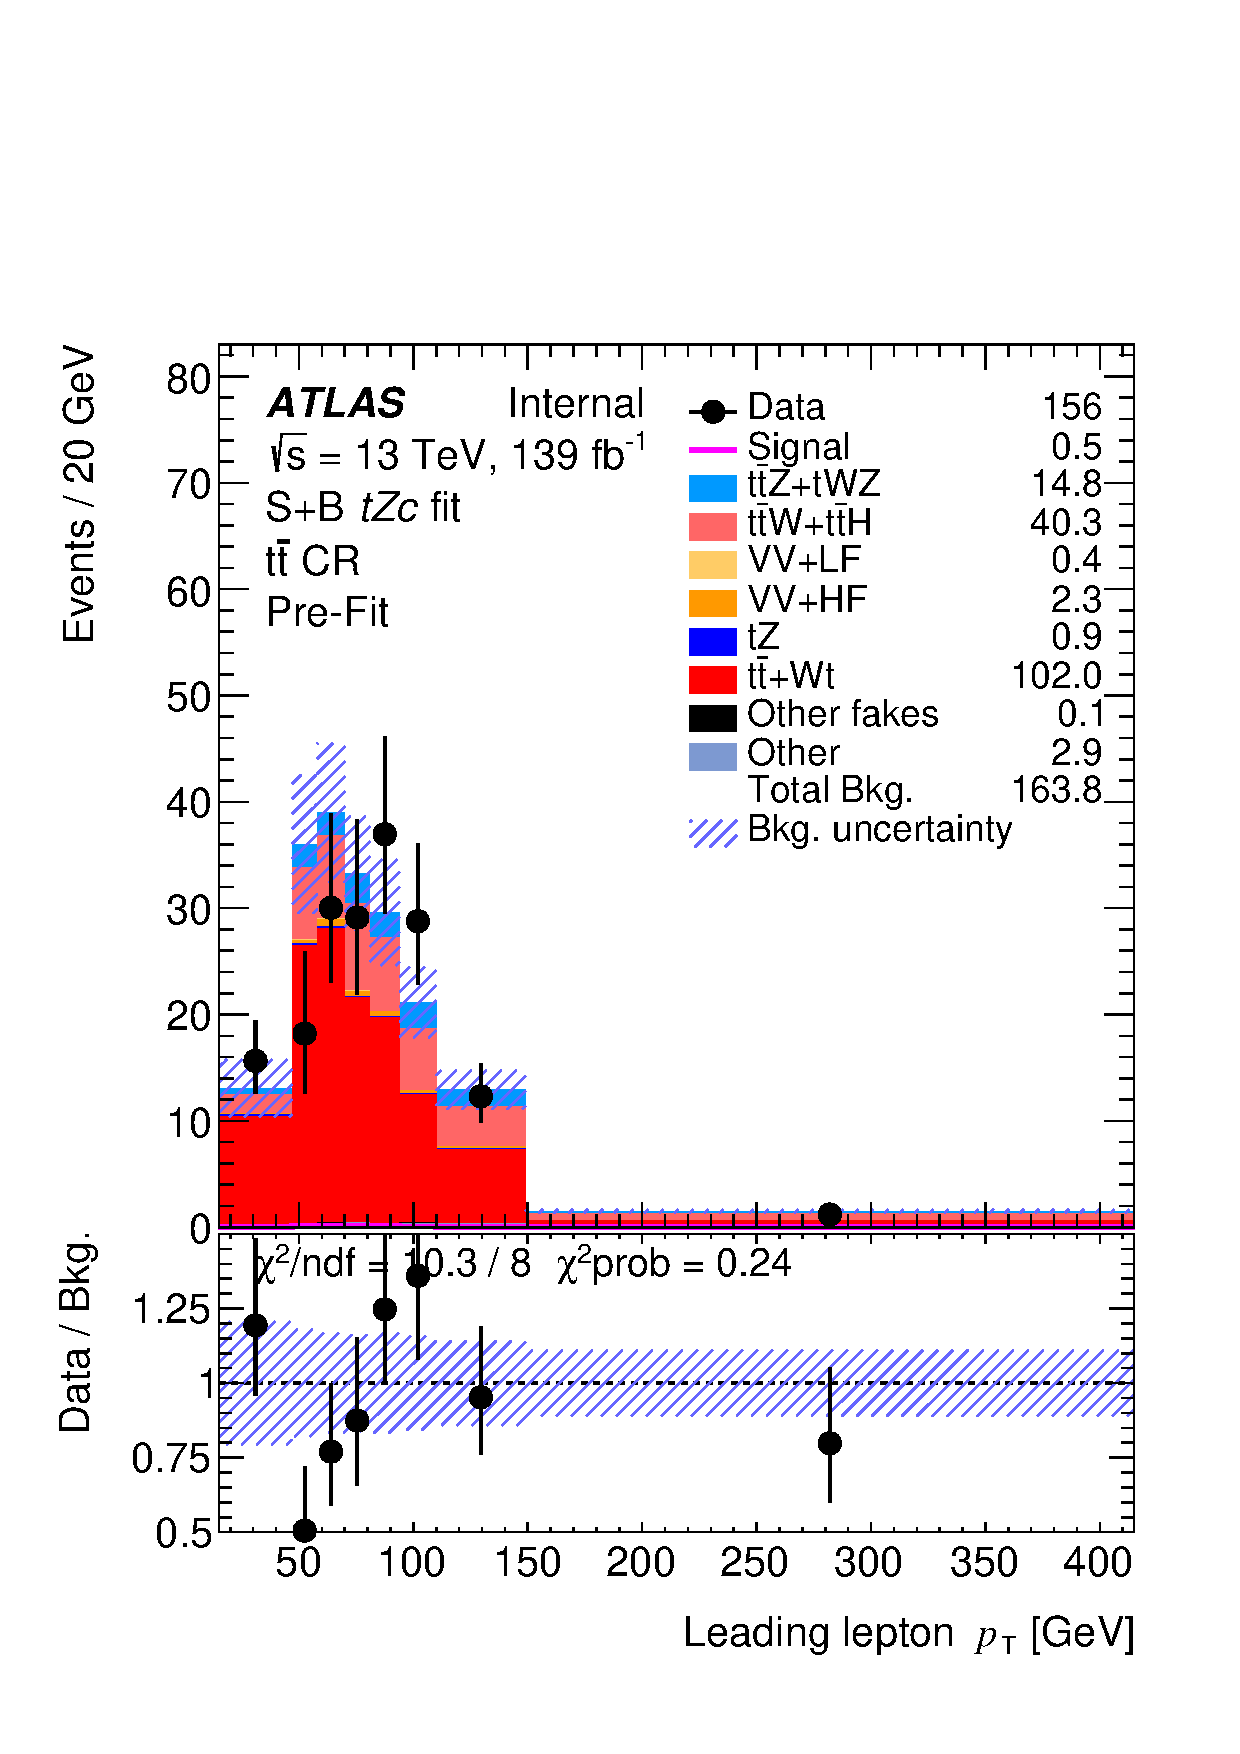
\includegraphics[width=.45\textwidth]{Appendices/AP9/figures/SPLUSB_CRSR_UsingBaseFullSys/Plots/TTCR} &
		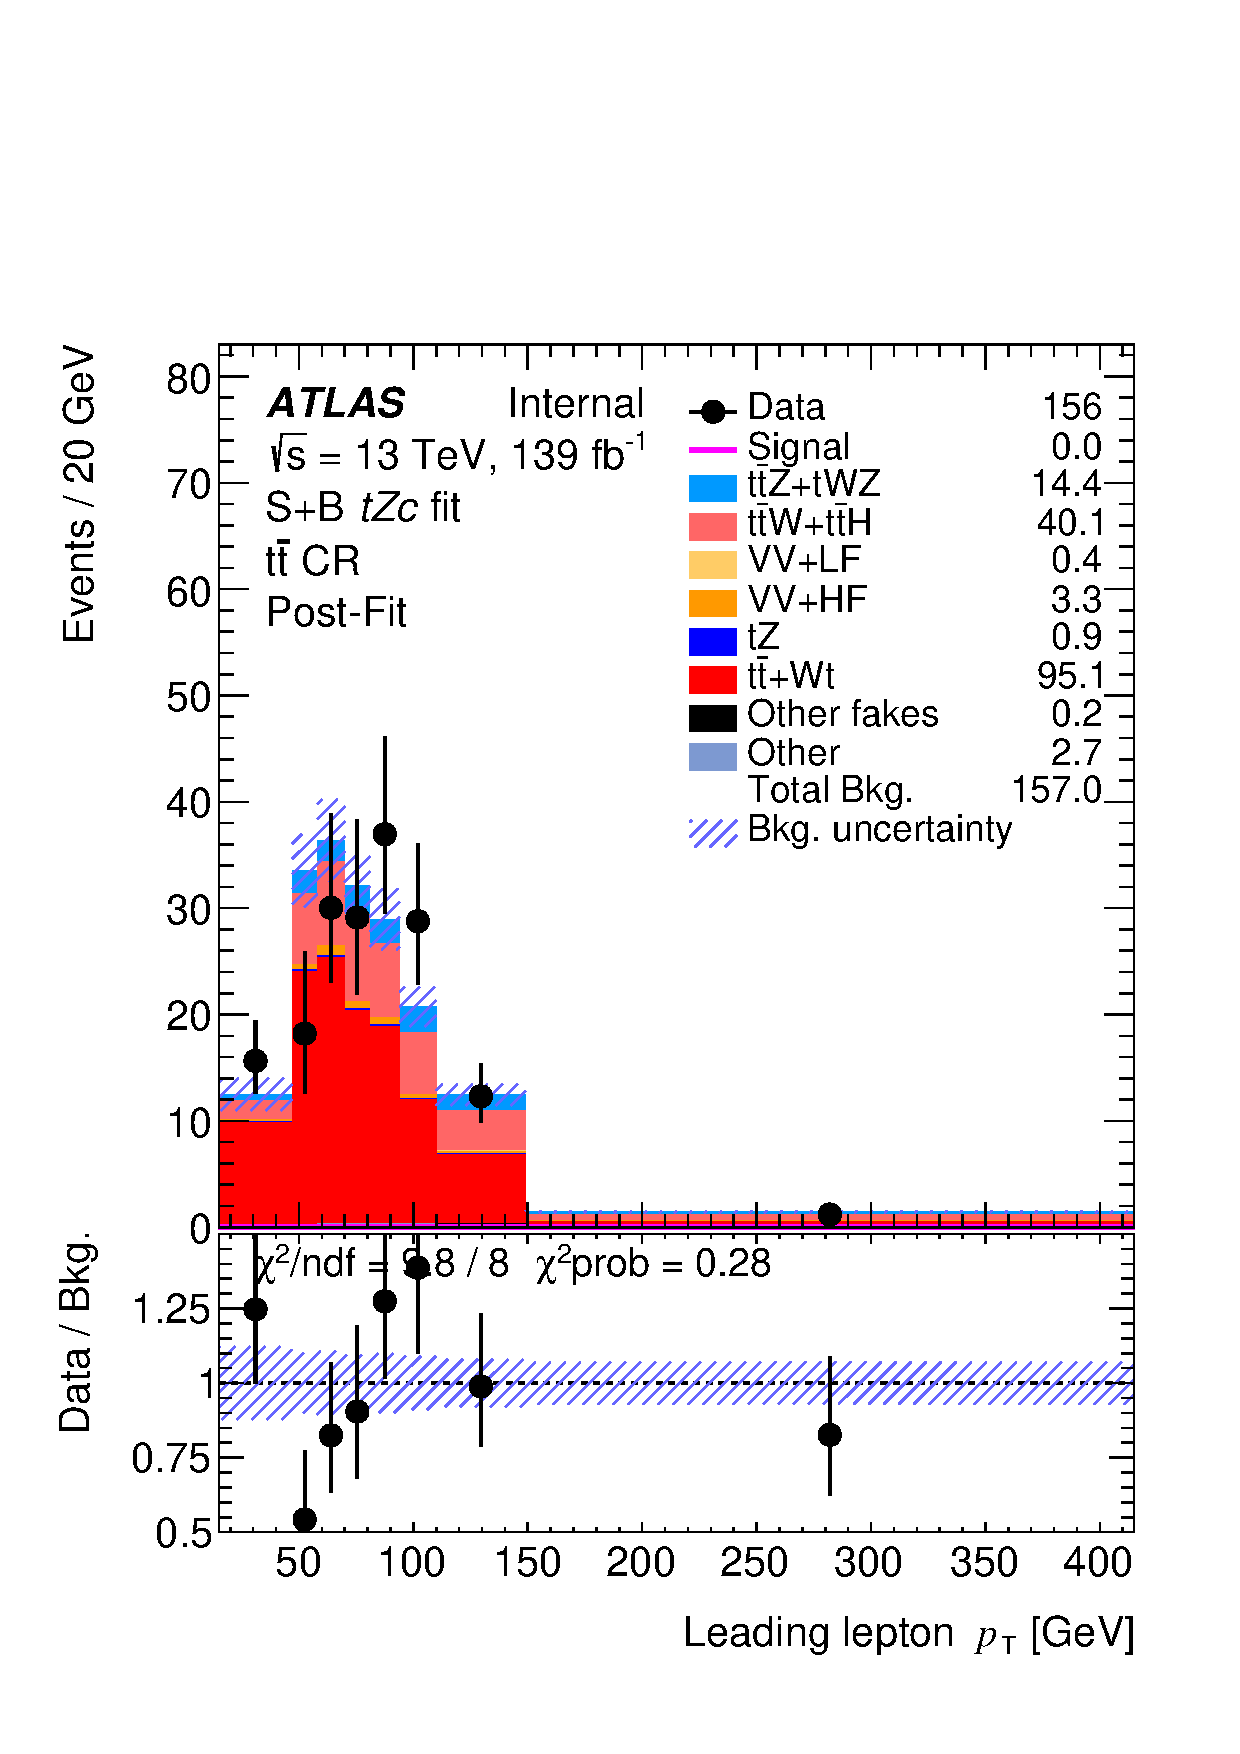
\includegraphics[width=.45\textwidth]{Appendices/AP9/figures/SPLUSB_CRSR_UsingBaseFullSys/Plots/TTCR_postFit} \\
		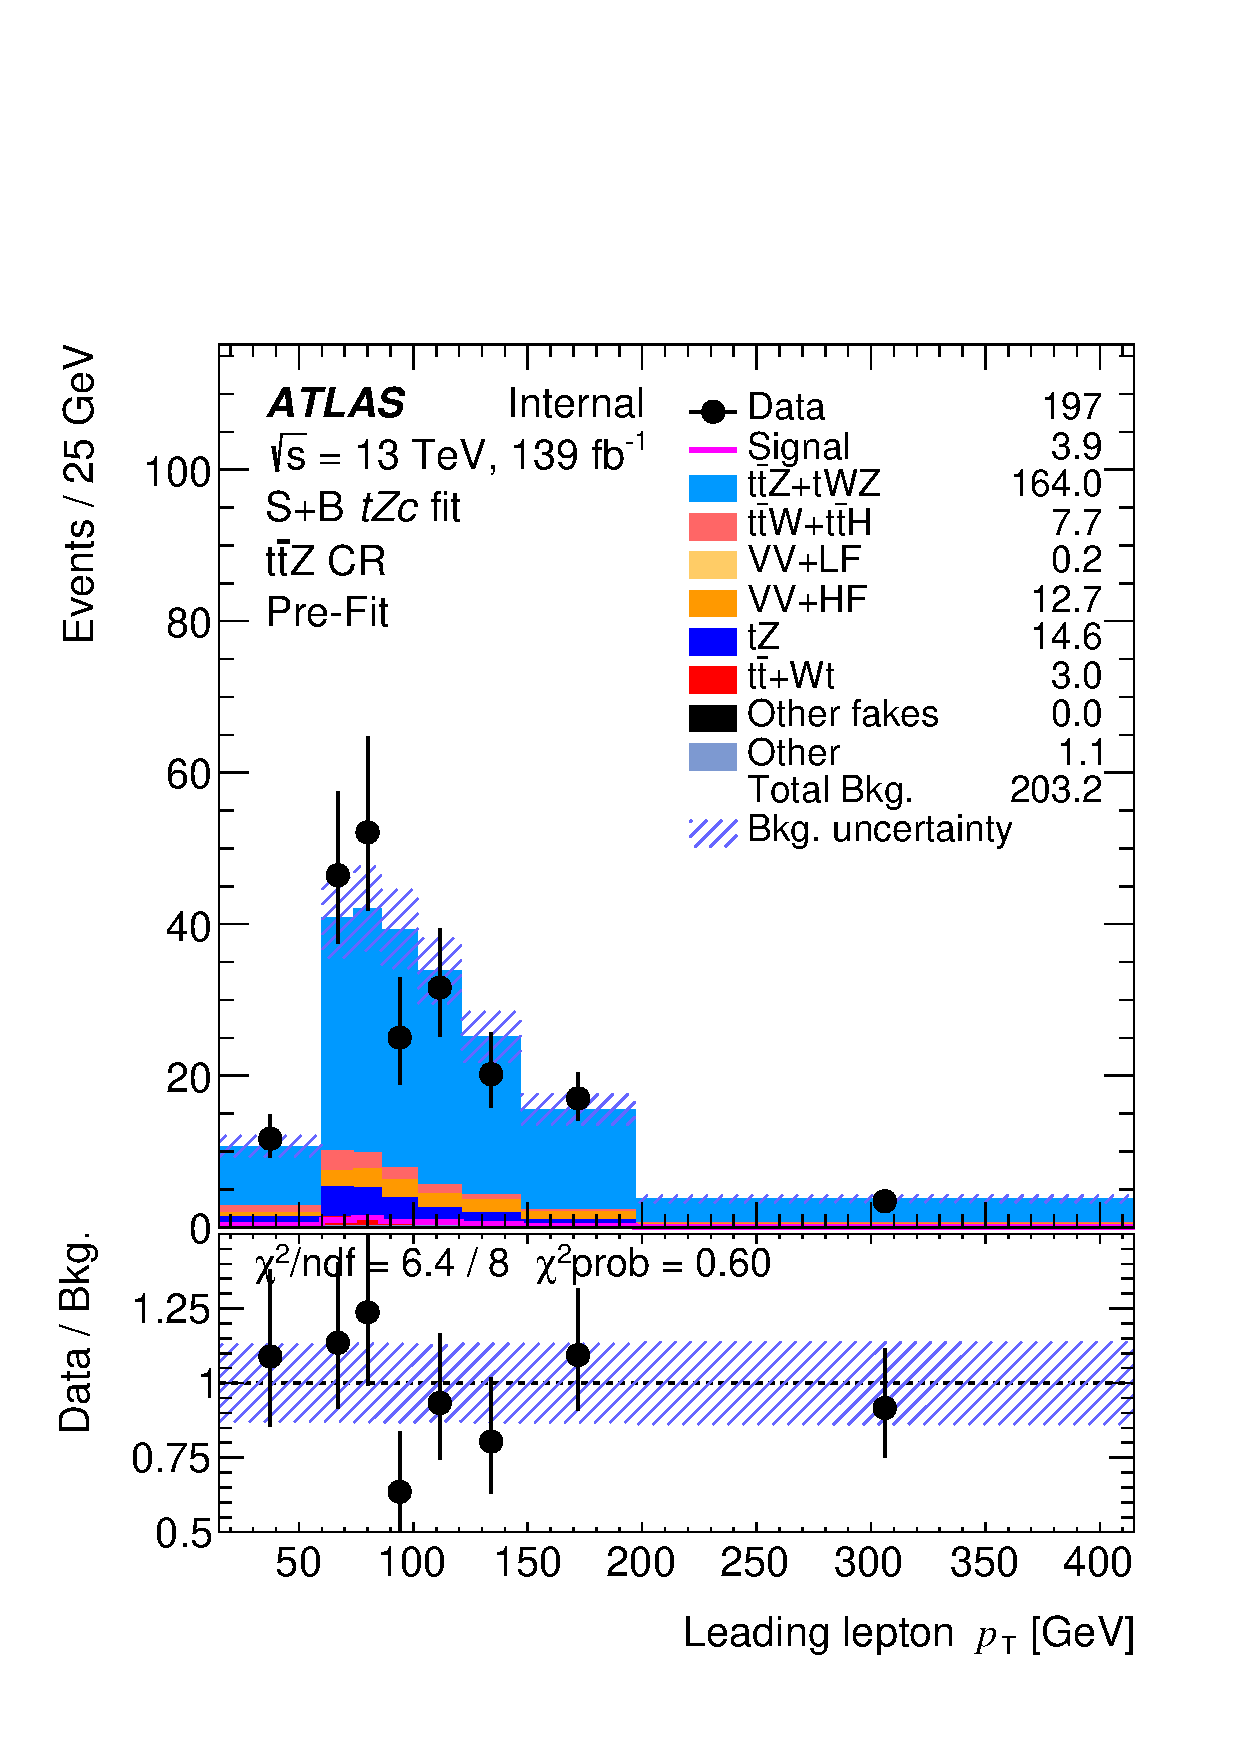
\includegraphics[width=.45\textwidth]{Appendices/AP9/figures/SPLUSB_CRSR_UsingBaseFullSys/Plots/TTZCR} &
		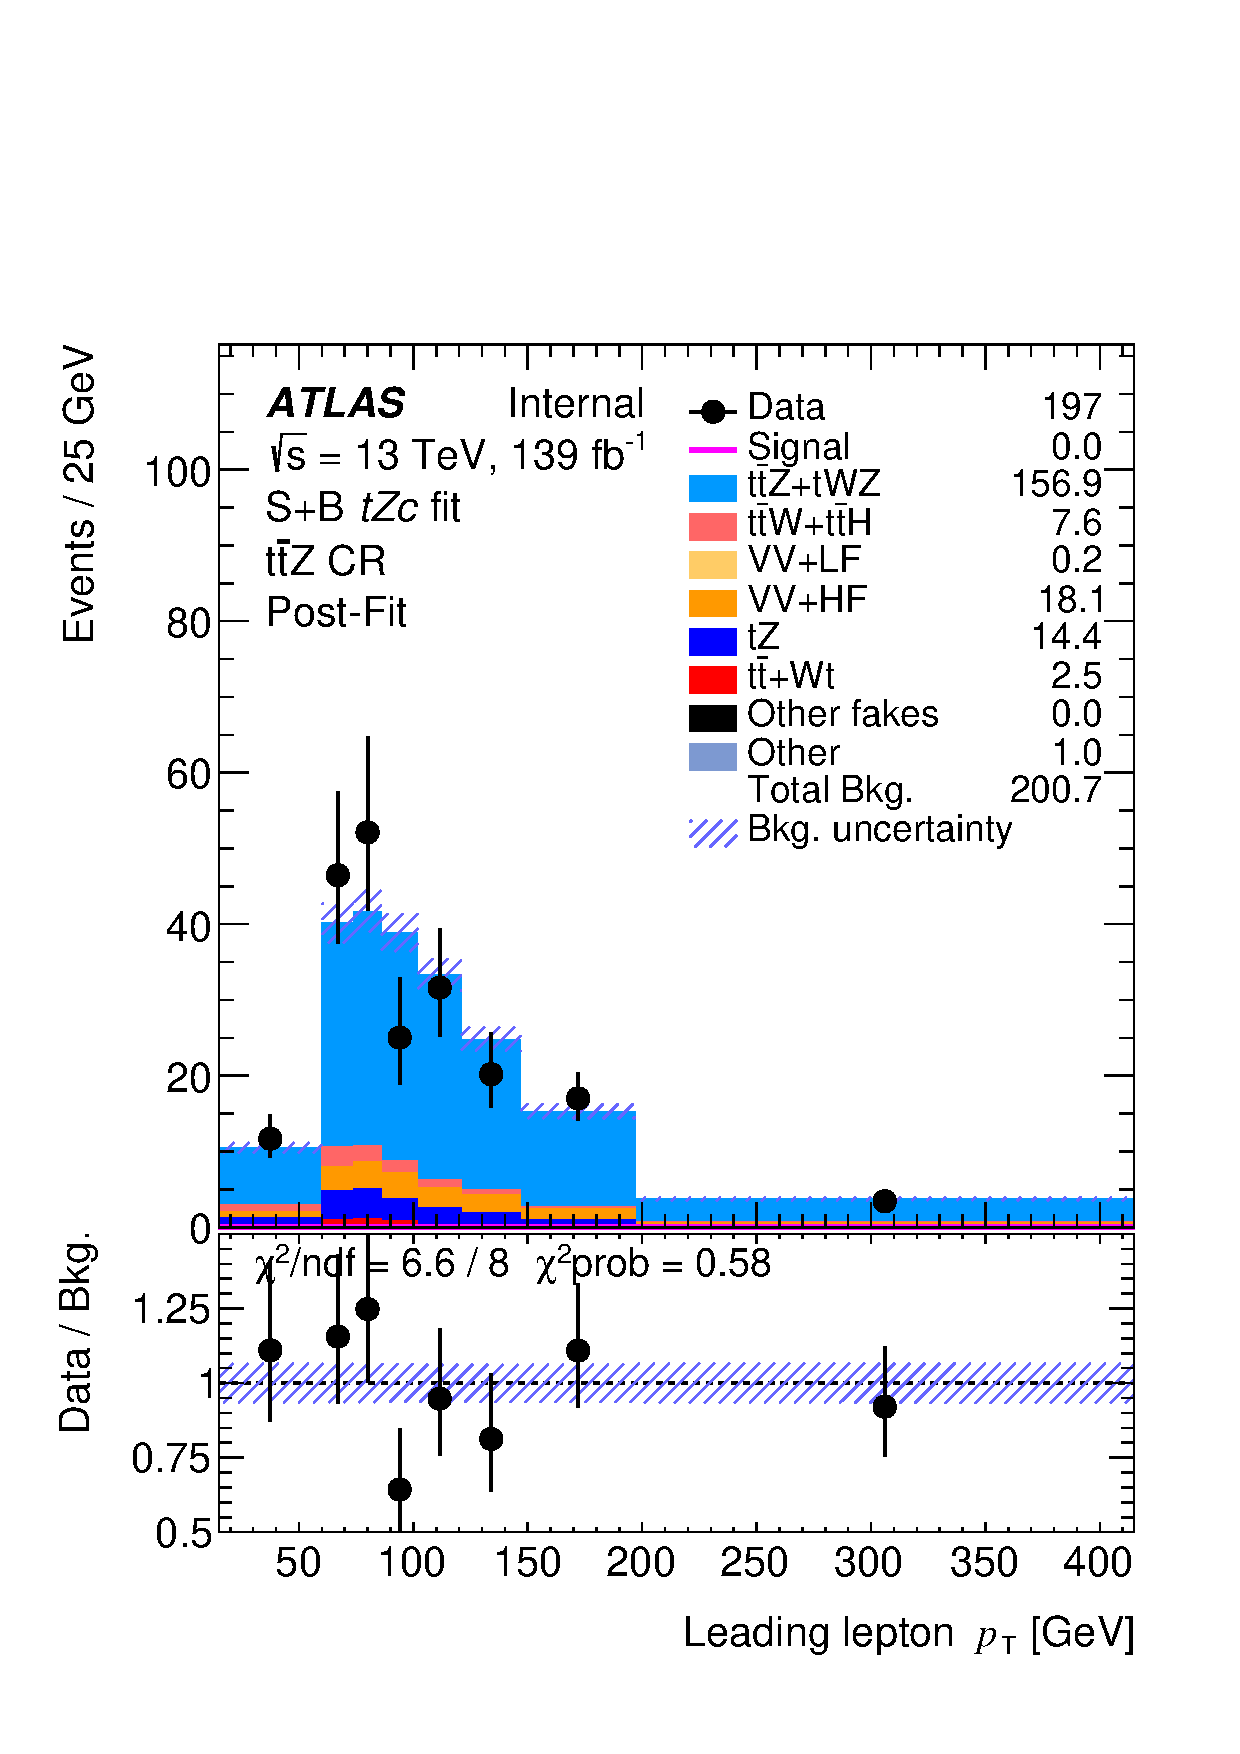
\includegraphics[width=.45\textwidth]{Appendices/AP9/figures/SPLUSB_CRSR_UsingBaseFullSys/Plots/TTZCR_postFit} \\
	\end{tabular}
	\caption{Pre-fit (left) and post-fit (right) leading lepton \pt distributions in the \ttbar and \ttZ CRs for the S+B \tZc fit in SRs+CRs with realistic Asimov.
		\ErrStatSys
	}%
	\label{fig:stat:tzc:splusb:crsr:crplots:2_base}
\end{figure}

\FloatBarrier
\noindent The expected upper limit, together
with the expected limit from the previous ATLAS
analysis~\cite{TOPQ-2017-06}, are reported in \Cref{tab:results:limits_base}.\\ 10.7 7.7 13.6
The limit from the previous analysis is improved by a factor of 3.
\begin{table}[htbp]
	\centering
	\begin{tabular}{lccc}
		\toprule
		\textbf{Limits} & \textbf{$-1\sigma$} & \textbf{Expected} & \textbf{$+1\sigma$} \\
		\midrule
		BR ($\Pqt\rightarrow\PZ\Pqc$) \cite{TOPQ-2017-06} & 22 & 32& 46 \\
		BR $\Pqt\rightarrow\PZ\Pqc$                                   & \SI{7.7e-5}{} & \SI{10.7e-5}{} & \SI{13.6e-5}{} \\
		\bottomrule
	\end{tabular}
	\caption{
		Expected limit on the branching ratios of $\Pqt\rightarrow\PZ\Pqc$ without using any c-tagger.
		Expected limit from \cite{TOPQ-2017-06} is also included for reference.
	}%
	\label{tab:results:limits_base}
\end{table}



